\section{Numerical Experiments}
	
	This section intends to be the most important in the chapter since it will take advantage of everything that has been previously studied and expand in the best possible way the implementation of the spectral methods studied in the previous section. For this, we will focus on the nonlinear problem defined in (\ref{IVP_Burgers}) directly, because after understanding these tools you want to have the ability to attack more complex problems such as (\ref{navierstokes}) which it is nonlinear, and in general, in most problems, it is not always possible to obtain analytical solutions, and then an option is to approximate them with numerical methods. \\
	
	According to what was studied in the previous section, we will start solving our problem with each method considering $\alpha> 0$, and later we will study the case when $\alpha = 0$. To find solutions we are going to use Euler's method, either explicit or implicit, to solve in the variable $t$, and due to the importance of carrying out numerical studies, we will try to give a detailed methodology about each method implemented to construct an algorithm that can be useful in the realization of computational codes. Finally, with the aim of giving a more detailed analysis, we will present some simulations of the results obtained.
	
	\subsection{Numerical Solutions for Burgers' Equation with Viscosity}
		\subsubsection{Simulations for Fourier-Galerkin Method}
		
		Following the ideas in the previous section for the Fourier-Galerkin method, we will assume that the expansion of the solution of (\ref{IVP_Burgers}) is as follows
		\begin{align*}
			u(x, t) = \displaystyle \sum_{|n| \leq \infty} \hat{u}_n (t) \phi_n (x), \hspace{2mm} \hat{u}_n (t) = \frac{1}{2 \pi} \left\langle u (x, t), \phi_n (x) \right\rangle,  
		\end{align*}
		and as before $\phi_n (x) = e^{inx}$. \\
	
		Similarly, we consider the space $V_N = \hat{B}_N \cap H^2_p (\mathcal{D})$ where we will look for its truncated expansion given by
		\begin{align*}
			u_N (x, t) = \displaystyle \sum_{ |n| \leq N } \hat{u}_n (t) \phi_n (x), \hspace{2mm} \hat{u}_n (t) = \frac{1}{2 \pi} \left\langle u (x, t), \phi_n (x) \right\rangle, 
		\end{align*}  
		which we are going to force to satisfy the following
		\begin{align}
			\left\langle R_N, \phi_n \right\rangle = \left\langle \frac{\partial u_N}{\partial t} + \frac{1}{2} (u_N^2)_x - \alpha \frac{\partial^2 u_N}{\partial x^2}, \phi_n \right\rangle = 0, \hspace{2mm}  \hspace{2mm} \phi_n \in V_N, \hspace{2mm} \forall t > 0
		\end{align}
		or equivalently
		\begin{align*}
			\displaystyle \int_{I} \frac{\partial}{\partial t} u_N (x, t) \overline{\phi_n (x)} dx = \alpha \int_{I} \frac{\partial^2}{\partial x^2} u_N(x, t) \overline{\phi_n (x)} dx - \int_{I} \frac{1}{2} \frac{\partial}{\partial x} \left[ u_N(x, t) \right]^2 \overline{\phi_n (x)} dx   
		\end{align*}
		Since $u_N (x, t)$ and its derivatives are periodic in space, integrating by parts we obtain that
		\begin{align*}
			\displaystyle \int_{I} \frac{\partial}{\partial t} u_N (x, t) \overline{\phi_n (x)} dx = - \alpha \int_{I} \frac{\partial}{\partial x} u_N(x, t) \frac{\partial}{\partial x} \overline{\phi_n (x)} dx + \int_{I} \frac{1}{2} \left[ u_N(x, t) \right]^2 \frac{\partial}{\partial x} \overline{\phi_n (x)} dx   
		\end{align*} 
		
		Then writing again as an inner product
		\begin{align*}
			\left\langle \frac{\partial u_N}{\partial t}, \phi_n  \right\rangle = \left\langle - \alpha \frac{\partial u_N}{\partial x} + \frac{1}{2} [u_N]^2, \frac{\partial \phi_n}{\partial x}  \right\rangle
		\end{align*}
		and using the orthogonality $\langle \phi_l, \phi_n \rangle = 2 \pi \delta_{ln}$, for each $n$ fixed we have to
		\begin{align*}
			\left\langle \frac{\partial u_N}{\partial t}, \phi_n  \right\rangle = \left\langle \displaystyle \sum_{ |l| \leq N} \frac{d \hat{u}_l (t)}{dt} \phi_l, \phi_n  \right\rangle = 2 \pi \frac{d \hat{u}_n (t)}{dt}
		\end{align*}
		
		\noindent and for the other terms
		\begin{align*}
			\left\langle \frac{\partial u_N}{\partial x} - \frac{1}{2} [u_N]^2, \frac{\partial \phi_n}{\partial x}  \right\rangle = & \alpha \left\langle - i \displaystyle \sum_{ |l| \leq N} l \hat{u}_l (t) \phi_l, in \phi_n \right\rangle \\
			&+ \left\langle\frac{1}{2} \left( \sum_{ |p| \leq N} \hat{u}_p (t) \phi_p \right) \left( \sum_{ |q| \leq N} \hat{u}_q (t) \phi_q \right), in \phi_n \right\rangle \\
			=&  - \alpha n \left\langle  \displaystyle \sum_{ |l| \leq N} l \hat{u}_l (t) \phi_l, \phi_n \right\rangle - \frac{in}{2} \left\langle \sum_{ |p| \leq N} \sum_{ |q| \leq N} \hat{u}_p (t) \hat{u}_q (t) \phi_{p + q}, \phi_n \right \rangle \\
			=& -2 \pi \alpha n^2 \hat{u}_n (t) - in \pi \sum_{ p + q = n} \hat{u}_p (t) \hat{u}_q (t), \hspace{2mm} |q|, |p| \leq N.
		\end{align*}
		
		\noindent Therefore, using the linear transformation from $\mathcal{D}_p = [0, 2 \pi]$ to $\mathcal{D} = [x_L, x_R]$ given by $x = P z + x_L$ to escalate the problem, where $P = \frac{x_R - x_L}{2 \pi}$ and $z \in \mathcal{D}_p$, we have the following system of nonlinear ordinary differential equations
		\begin{align}
		\label{Galerkin_Nonlinear}	
			\frac{d \hat{u}_n (t)}{dt} = - \alpha P^2 n^2 \hat{u}_n (t) - \frac{in}{2} P \sum_{ p + q = n} \hat{u}_p (t) \hat{u}_q (t), \hspace{2mm} |q|, |p| \leq N, 
		\end{align}
		or equivalently
		\begin{align*}
			\frac{d \hat{u}_n (t)}{dt} = - \alpha P^2 n^2 \hat{u}_n (t) - \frac{in}{2} P \sum_{|q| \leq N} \hat{u}_{n - q} (t) \hat{u}_q (t), \hspace{2mm} |n| \leq N, 
		\end{align*}
		which is solved using the initial condition of the original projected problem on the space $V_N$, that is,
		\begin{align*}
			\mathcal{P}_N u_0 = \displaystyle \sum_{|n| \leq N} a_n \phi_n (x), \hspace{2mm} a_n = \frac{1}{2 \pi} \langle u_0 (x), \phi_n (x) \rangle.   
		\end{align*}
		
		This problem can be treated in different ways and, in this work, we will develop it with the following approach. First, let's discard the terms $\hat{u}_q$ such that $|q| > N$ on the right side of the equation above, to get the following
		\begin{align*}
			\frac{d \hat{u}_n (t)}{dt} =  -\alpha P^2 n^2 \hat{u}_n (t) - \frac{in}{2} P \sum_{|q| \leq N} \hat{u}_{n - q} (t) \hat{u}_q (t), \hspace{2mm} |n - q| \leq N , 
		\end{align*}
		which is a system of $2N + 1$ equations. \\
		
		There is a wide variety of numerical methods to solve the above problem, and since this is not linear, it is not easy to justify choosing an appropriate method, since advanced knowledge of numerical analysis is required to investigate its characteristics. The way to choose a candidate method is by investigating its numerical stability, which guarantees that the numerical solution does not explode towards infinity and that it is at least bounded. \\
		
		In general, explicit methods are not suitable for nonlinear problems and are commonly handled by implicit methods. To show the implementation, and in addition to looking at its most relevant characteristics, we will solve the problem using Euler's implicit method. First, note that when $n = 0$ we have $\hat{u}_0 (t) = \hat{u}_0 (0)$, and that the nonlinear term involves the term $\hat{u}_n$ only when $q = 0$. So, using the integrating factor $e^{\lambda_n t}$ with $\lambda_n = \alpha P^2 n^2 + \frac{in}{2} P \hat{u}_0 (0) $ we can obtain the following formulation
		\begin{align*}
			\frac{d \left[ e^{\lambda_n t} \right]  \hat{u}_n (t)}{dt} = - \frac{in}{2} P e^{ \lambda_n t} \left[ \hat{u}_0 (0) \hat{u}_n (t) + \sum_{\substack{|q|\leq N \\ q \neq 0, n}} \hat{u}_{n - q} (t) \hat{u}_q (t) \right],
		\end{align*}	
		and its solution using implicit Euler
		\begin{align*}
			\hat{u}^{j+1}_n = e^{- \lambda_n \Delta t} \left[ \hat{u}^j_n - \Delta t \frac{in}{2} P \sum_{\substack{|q|\leq N \\ q \neq 0, n}} \hat{u}^{j}_{n - q} \hat{u}^{j}_q \right] - \Delta t \frac{in}{2} P \hat{u}_0 (0) \hat{u}^{j+1}_n, 
		\end{align*}
		and then solving for the term $\hat{u}^{j + 1}_n$ to obtain
		\begin{align*}
			\hat{u}^{j+1}_n &= \frac{ e^{- \lambda_n \Delta t}}{ 1 + \Delta t \frac{in}{2} P \hat{u}_0 (0) } \left[ \hat{u}^j_n - \Delta t \frac{in}{2} P \sum_{\substack{|q|\leq N \\ q \neq 0, n}} \hat{u}^{j}_{n - q} \hat{u}^{j}_q \right].   
		\end{align*}	
		
		Furthermore, using this formulation repeatedly for each $j$ gives us
		\begin{align}
		\label{Galerkin_Euler}
			\hat{u}^{j+1}_n &= \left[ \frac{ e^{- \lambda_n \Delta t}}{ 1 + \Delta t \frac{in}{2} P \hat{u}_0 (0) } \right]^{j+1} \hat{u}^0_n - \Delta t \frac{in}{2} P \sum_{k=1}^{j+1} \left[ \frac{ e^{- \lambda_n \Delta t}}{ 1 + \Delta t \frac{in}{2} P \hat{u}_0 (0) } \right]^{k}  \sum_{\substack{|q|\leq N \\ q \neq 0, n}} \hat{u}^{j+1-k}_{n - q} \hat{u}^{j+1-k}_q
		\end{align}
		Now, we will proceed to describe the steps necessary to implement the method based on the above. The simulations we are going to show were based on the formulation (\ref{Galerkin_Euler}), taking advantage of the fast Fourier transformation to calculate the coefficients $\hat{u}_n$, since it allows us to go from physical space to the space of Fourier and conversely. Also, it is worth mentioning that the codes used in this work can be found at \url{https://github.com/alanmatzumiya/pySpectralPDE.git}. \\ 
		
		To carry out these numerical experiments it was necessary to follow the following steps:
		\begin{enumerate}
			\item Set the intervals to consider, $[x_L, x_R]$ for physical space and $[t_0, t_f]$ for time, and give an initial condition function $u_0$. It is also necessary to choose the value of $N$, and another for the parameter $\alpha$. 
			
			\item We proceed to calculate the points in the spatial grid where we want to obtain the solution, and for this, we define the points $z_i \in [0, 2 \pi]$ as
			\begin{align*}
				z_i = \frac{2 \pi i}{N}, \hspace{2mm} i = 0, 1, \dots, N
			\end{align*}
			which are used to obtain the points $x_i \in [x_L, x_R]$
			\begin{align*}
				x_i = P z_i + x_L, \hspace{2mm} P = \frac{x_R - x_L}{2 \pi}
			\end{align*}
			
			To obtain the points $t_j \in [t_0, t_f]$, we define the sequence $j = 0, 1, \dots, M$, for some positive $M$, and calculate the following
			\begin{align*}
				t_j = t_0 + j \Delta t, \hspace{2mm} \Delta t = \frac{t_f - t_0}{M} 
			\end{align*}
			
			The values $| n | = 0, 1, \dots, N $ must be established to calculate $in, n^2$, which are required to approximate the derivatives.
			 
			\item Calculate the coefficients $\hat{u}_0$ of the initial condition function $u_0$, using the fast Fourier transformation based on the already fixed spatial grid. So, it is possible to start the recursive rule given by (\ref{Galerkin_Euler}) for every $t_j$.
			
			\item Finally, the approximation obtained is evaluated using the equation given by
			\begin{align*}
				u_N(x, t_j) = \displaystyle \sum_{|n| \leq N} \hat{u}_n (t_j) e^{inx}.
			\end{align*}
		\end{enumerate}
		
		For the numerical study, we will establish the following initial condition
		\begin{align}
			\label{IC}
			u_0 (x) = e^{0.05 x^2}, \hspace{3mm} x \in [x_L, x_R] 
		\end{align}	
		
		To compare results, we will use the approximation given by (\ref{Exact_Solution_Approximation}) as the exact solution. In the figure \ref{Galerkin_alphas} shows the maximum distance over every $t \in [0, 100]$ between the exact solution and its approximations given by (\ref{Galerkin_Euler}) for $N = 2^m$, $m = 4, \dots, 12$, $\Delta t = 1.0 \times 10^{-5}$, and different values of $\alpha$. Furthermore, in Tables \ref{Galerkin_tabla_L2_alpha=1} and \ref{Galerkin_tabla_max_alpha=1}, we can see the numerical values ​​of these distances for different configurations of $N$ and $\Delta t$. Similarly, in Tables \ref{Galerkin_tabla_L2_alpha=005} and \ref{Galerkin_tabla_max_alpha=005} but for $\alpha = 0.005$.
	
	\begin{figure}[H]
		\centering
		\includegraphics[width=15cm]{burgers_equation/deterministic/numerical_experiments/viscid/figures/galerkin/alphas_Error_N.png}
		\caption{(a) $L^2$-norm between the exact solution and its approximations using Galerkin method. (b) Max norm between the exact solution and its approximations.}
		\label{Galerkin_alphas}
	\end{figure}
	\newpage
	\begin{figure}[H]
		\centering
		\caption{Numerical solution for (\ref{IVP_Burgers}) using (\ref{Galerkin_Euler}) with $\alpha = 1.0$, $N=2048$, and $\Delta t = 1.0 \times 10^{-5}$.}
		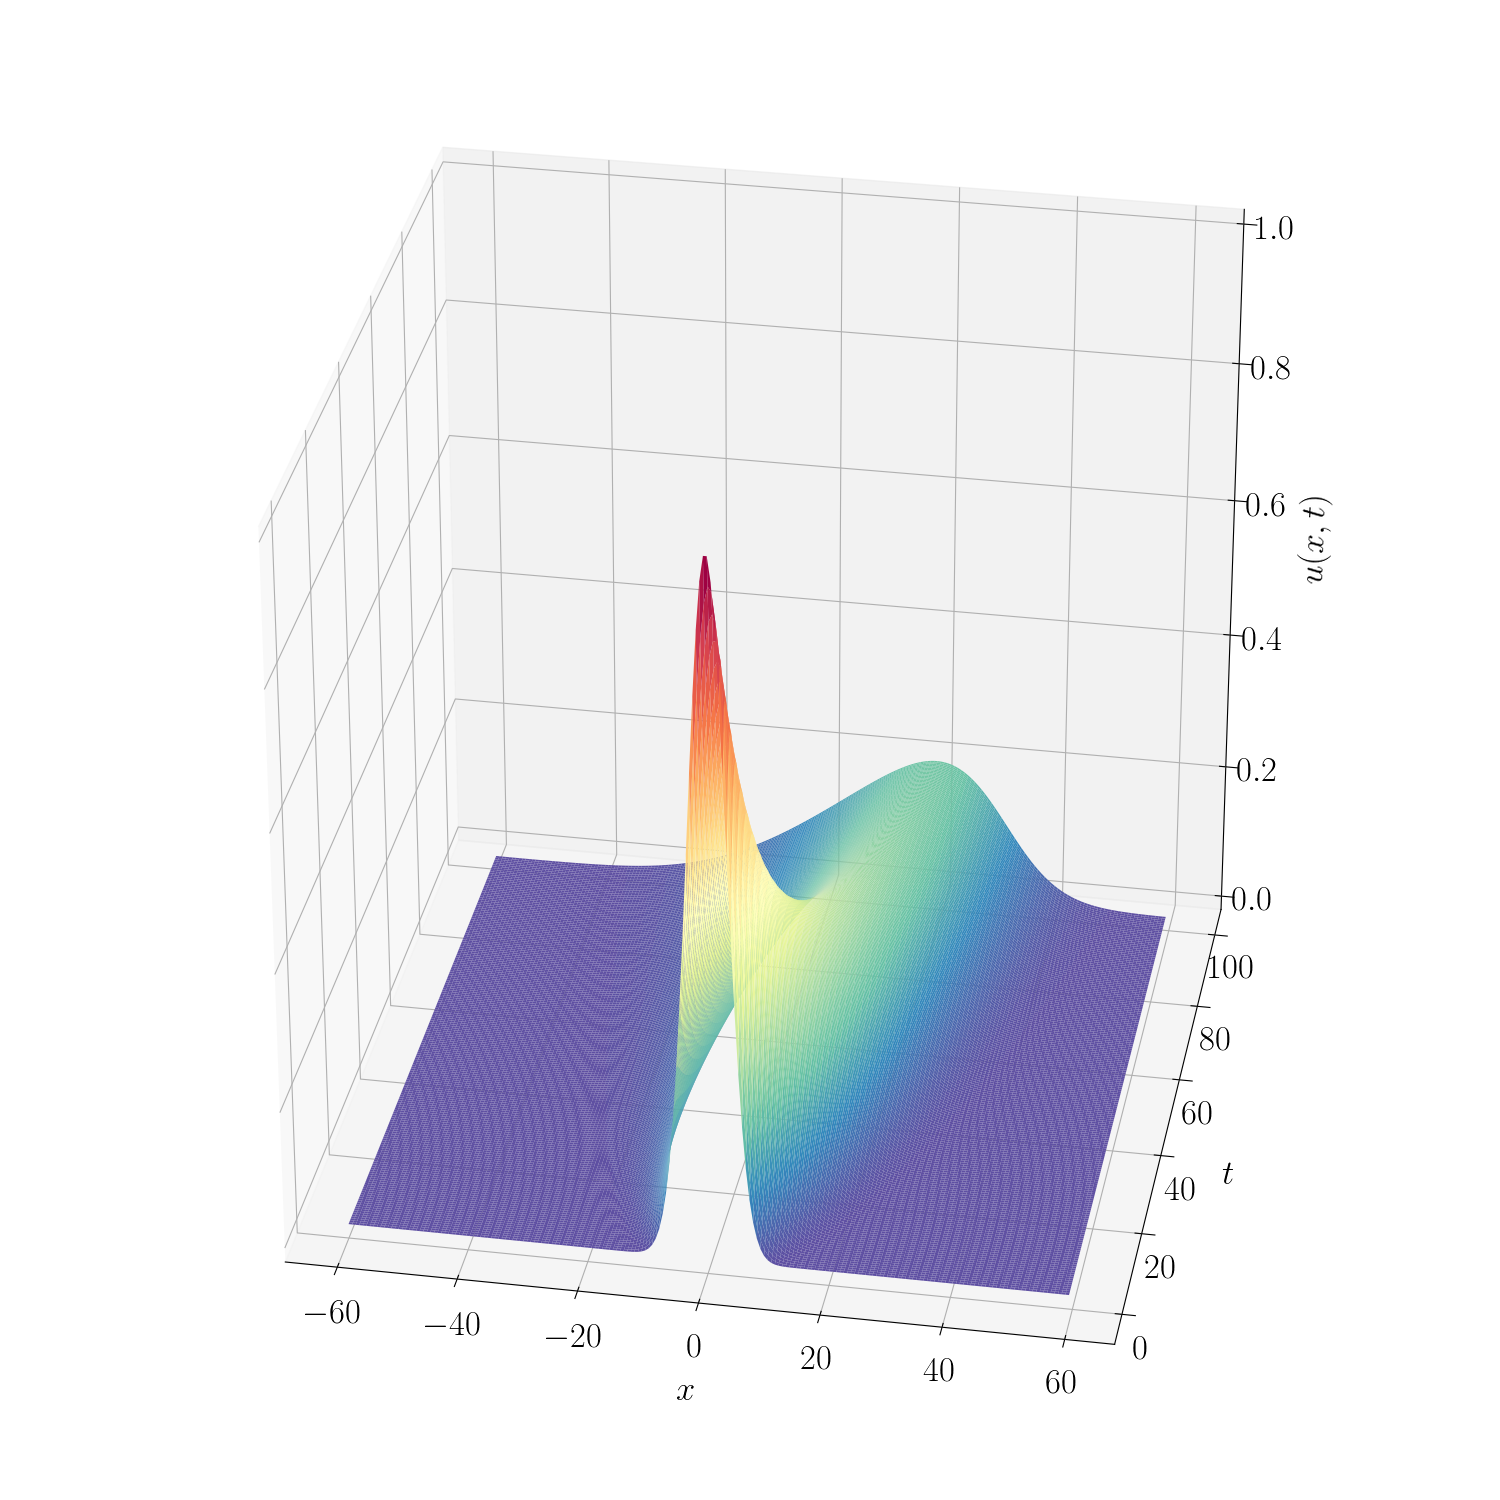
\includegraphics[width=12cm]{burgers_equation/deterministic/numerical_experiments/viscid/figures/galerkin/Numerical_Solution_alpha=1.png}
		\label{Galerkin_alpha=1}
		\caption{Numerical solution for (\ref{IVP_Burgers}) using (\ref{Galerkin_Euler}) at the time $T = 100$ with $\alpha = 1.0$, and $\Delta t = 1.0 \times 10^{-5}$. (b) Point-wise error of approximation}
		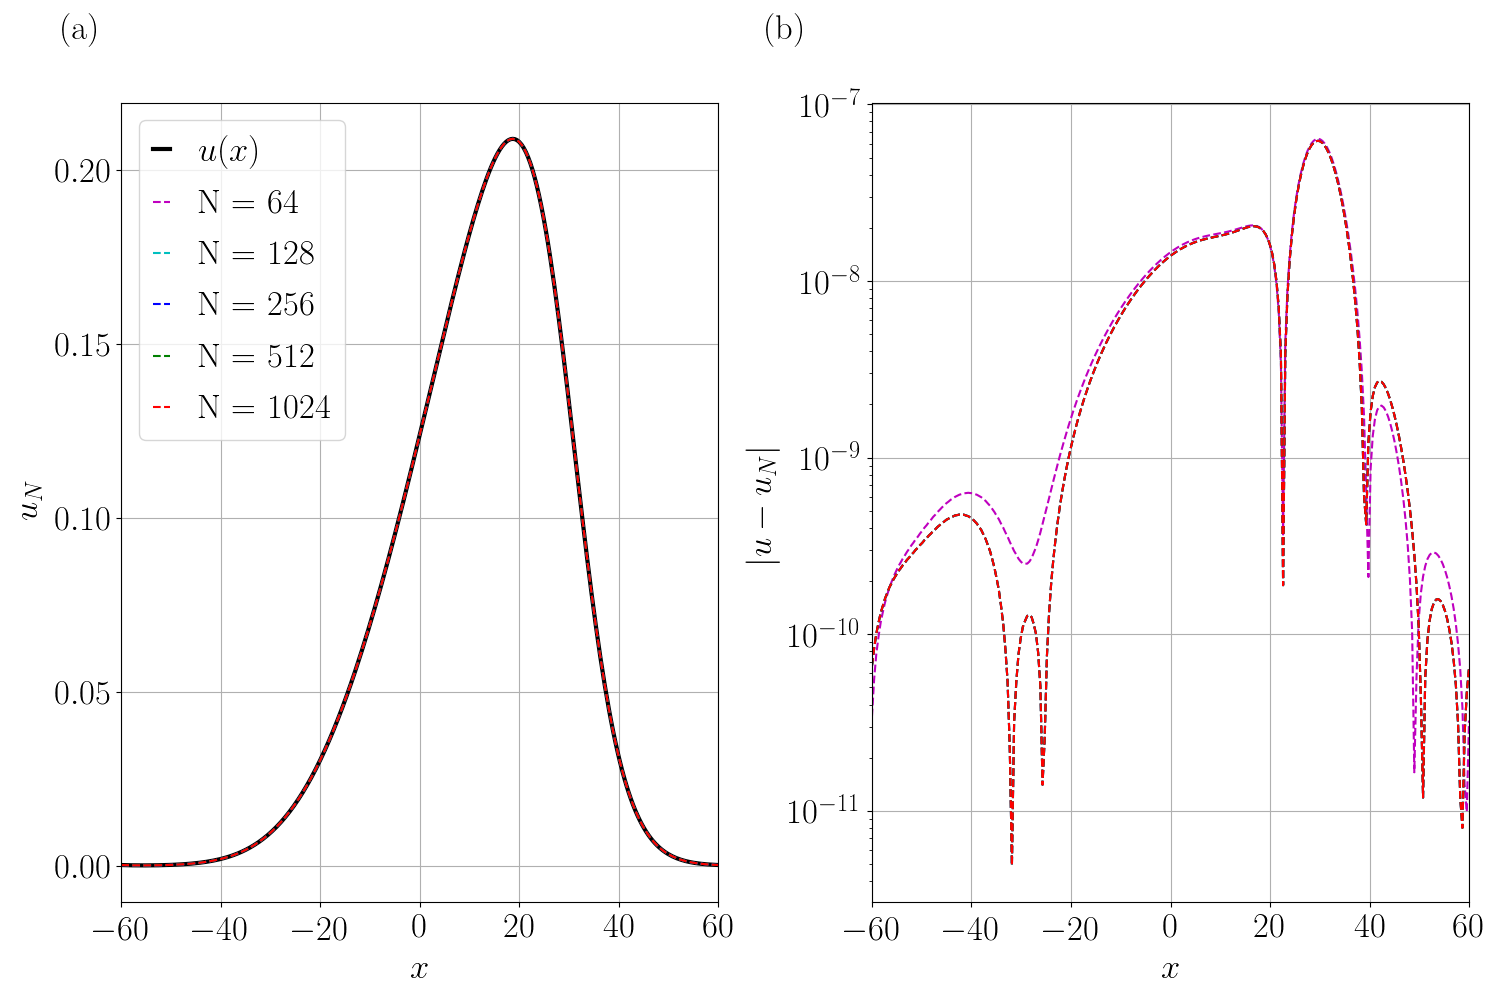
\includegraphics[width=12.5cm]{burgers_equation/deterministic/numerical_experiments/viscid/figures/galerkin/Numerical_Solution_alpha=1_T=100.png}
		\label{Galerkin_alpha=1_T}
	\end{figure}
	\begin{table}[H]
		\begin{tabular}{lcccc}
			\toprule
			\multicolumn{1}{c}{\textbf{Expansion}} & \multicolumn{4}{c}{\textbf{Error}} \\
			$\hspace{9mm}N$ & $\Delta t=1\times 10^{-2}$ & $\Delta t=1\times 10^{-3}$ & $\Delta t=1\times 10^{-4}$ & $\Delta t=1\times 10^{-5}$ \\
			\midrule
			\hspace{7mm} 16 & 0.72504    & 0.72504    & 0.72504    & 0.72504    \\
			\midrule
			\hspace{7mm} 32 & 6.90249 $\times 10 ^{-2}$   & 6.88052 $\times 10 ^{-2}$   & 6.87838 $\times 10 ^{-2}$   & 6.87816 $\times 10 ^{-2}$   \\
			\midrule
			\hspace{7mm} 64 & 1.23827 $\times 10 ^{-3}$  & 8.85367 $\times 10 ^{-4}$ & 8.80521 $\times 10 ^{-4}$ & 8.80410 $\times 10 ^{-4}$  \\
			\midrule
			\hspace{7mm} 128 & 9.43454 $\times 10 ^{-4}$ & 9.41793 $\times 10 ^{-5}$ & 9.41148 $\times 10 ^{-6}$ & 9.41827 $\times 10 ^{-7}$  \\
			\midrule
			\hspace{7mm} 256 & 9.43454 $\times 10 ^{-4}$ & 9.41793 $\times 10 ^{-5}$ & 9.41109 $\times 10 ^{-6}$ & 9.36411 $\times 10 ^{-7}$ \\
			\midrule
			\hspace{7mm} 512 & 9.43454 $\times 10 ^{-4}$ & 9.41793 $\times 10 ^{-5}$ & 9.41109 $\times 10 ^{-6}$ & 9.36411 $\times 10 ^{-7}$ \\
			\midrule
			\hspace{7mm} 1024 & $\ast$ & 9.41793 $\times 10^{-5}$ & 9.41109 $\times 10^{-6}$ & 9.36411 $\times 10^{-7}$              \\
			\midrule
			\hspace{7mm} 2048 & $\ast$ & $\ast$ & 9.41109 $\times 10^{-6}$ & 9.36411 $\times 10^{-7}$   \\
			\bottomrule
		\end{tabular}
		\caption{Error using $L^2$-norm with $\alpha = 1.0$}
		\label{Galerkin_tabla_L2_alpha=1}
		\vspace{1cm}
		\begin{tabular}{lcccc}
			\toprule
			\multicolumn{1}{c}{\textbf{Expansion}} & \multicolumn{4}{c}{\textbf{Error}} \\
			$\hspace{9mm}N$ & $\Delta t=1\times 10^{-2}$ & $\Delta t=1\times 10^{-3}$ & $\Delta t=1\times 10^{-4}$ & $\Delta t=1\times 10^{-5}$ \\
			\midrule
			\hspace{7mm} 16 & 0.203363    & 0.203333    & 0.203331    & 0.20333     \\
			\midrule
			\hspace{7mm} 32 & 2.64192 $\times 10 ^{-2}$   & 2.6248 $\times 10 ^{-2}$    & 2.62491 $\times 10 ^{-2}$  & 2.62492 $\times 10 ^{-2}$   \\
			\midrule
			\hspace{7mm} 64 & 6.93001 $\times 10 ^{-4}$ & 4.11641 $\times 10 ^{-4}$ & 3.85563 $\times 10 ^{-4}$ & 3.82972 $\times 10 ^{-4}$ \\
			\midrule
			\hspace{7mm} 128 & 4.74934 $\times 10 ^{-4}$ & 4.73649 $\times 10 ^{-5}$ & 4.74295 $\times 10 ^{-6}$ & 5.16105 $\times 10 ^{-7}$ \\
			\midrule
			\hspace{7mm} 256 & 4.74936 $\times 10 ^{-4}$ & 4.7368 $\times 10 ^{-5}$  & 4.72569 $\times 10 ^{-6}$ & 4.64922 $\times 10 ^{-7}$ \\
			\midrule
			\hspace{7mm} 512 & 4.74936 $\times 10 ^{-4}$ & 4.7368 $\times 10 ^{-5}$  & 4.72569 $\times 10 ^{-6}$ & 4.64922 $\times 10 ^{-4}$ \\
			\midrule
			\hspace{7mm} 1024 & * & 4.7368 $\times 10 ^{-5}$  & 4.72569 $\times 10 ^{-6}$ & 4.64922 $\times 10 ^{-7}$ \\
			\midrule
			\hspace{7mm} 2048 & * & * & 4.72569 $\times 10 ^{-6}$ & 4.64922 $\times 10 ^{-7}$ \\
			\bottomrule
		\end{tabular}
		\caption{Error using Max norm with $\alpha = 1.0$}
		\label{Galerkin_tabla_max_alpha=1}
	\end{table}

	\begin{figure}[H]
		\centering
		\caption{Numerical solution for (\ref{IVP_Burgers}) using (\ref{Galerkin_Euler}) with $\alpha = 0.005$, $N=2048$, and $\Delta t = 1.0 \times 10^{-5}$.}
		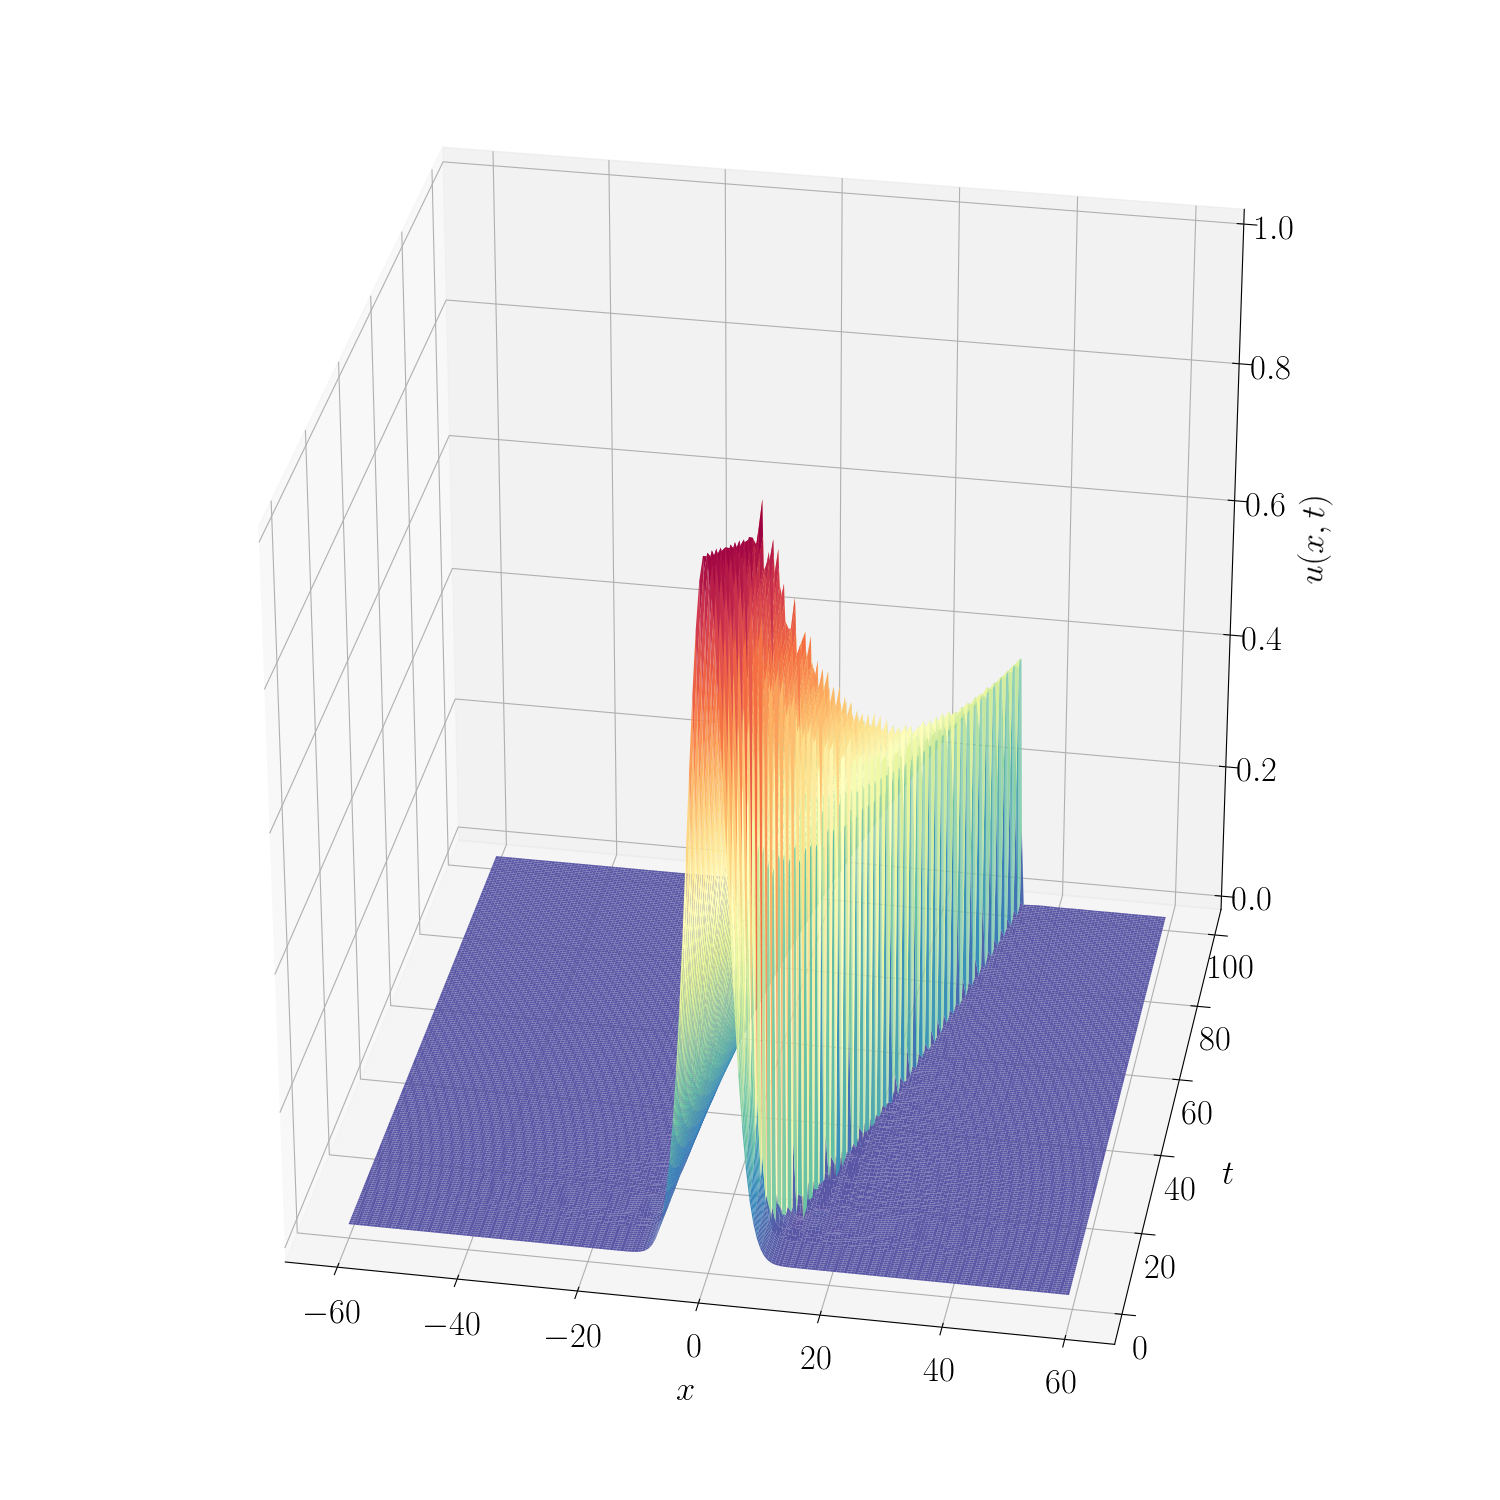
\includegraphics[width=12cm]{burgers_equation/deterministic/numerical_experiments/viscid/figures/galerkin/Numerical_Solution_alpha=0005.png}
		\caption{Numerical solution for (\ref{IVP_Burgers}) using (\ref{Galerkin_Euler}) at the time $T = 100$ with $\alpha = 1.0$, and $\Delta t = 1.0 \times 10^{-5}$. (b) Point-wise error of approximation}
		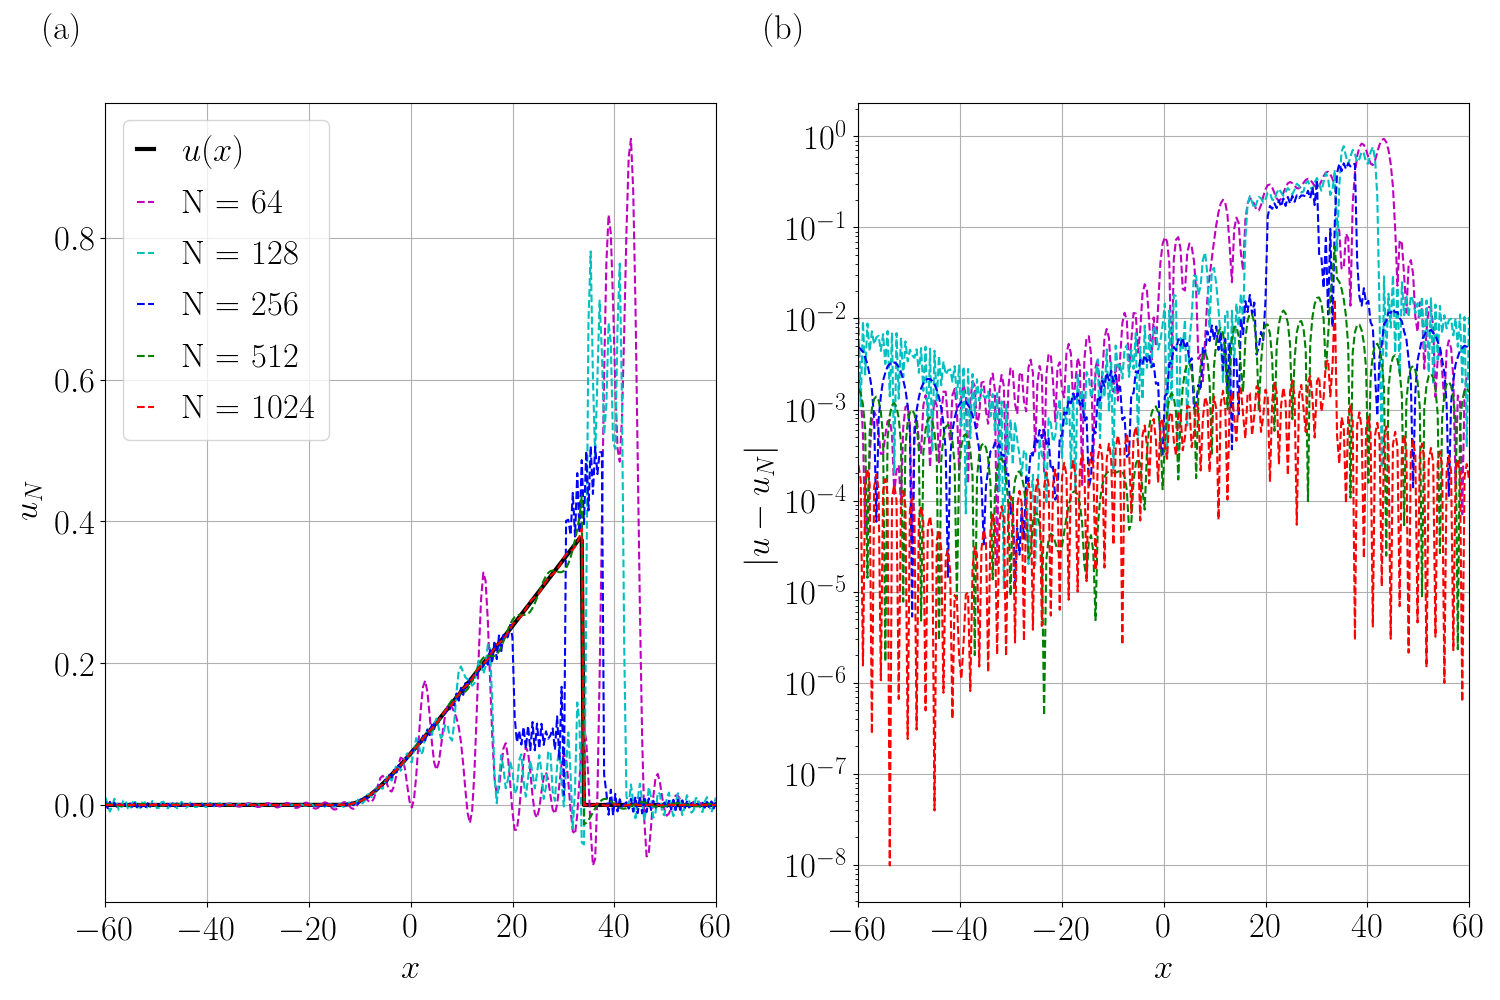
\includegraphics[width=12.5cm]{burgers_equation/deterministic/numerical_experiments/viscid/figures/galerkin/Numerical_Solution_alpha=0005_T=100.png}
		\label{Galerkin_alpha=005_T}
	\end{figure}
	
	\begin{table}[H]
	\begin{tabular}{lcccc}
		\toprule
		\multicolumn{1}{c}{\textbf{Expansion}} & \multicolumn{4}{c}{\textbf{Error}} \\
		$\hspace{9mm}N$ & $\Delta t=1\times 10^{-2}$ & $\Delta t=1\times 10^{-3}$ & $\Delta t=1\times 10^{-4}$ & $\Delta t=1\times 10^{-5}$ \\
		\midrule
		\hspace{7mm} 16 & 9.95328   & 9.91901    & 9.91597    & 9.91567    \\
		\midrule
		\hspace{7mm} 32 & 2.72607   & 2.70558    & 2.70347    & 2.70326    \\
		\midrule
		\hspace{7mm} 64 & 2.50343   & 2.45988    & 2.45543    & 2.45497    \\
		\midrule
		\hspace{7mm} 128 & 2.16142   & 2.06992    & 2.05918    & 2.05795    \\
		\midrule
		\hspace{7mm} 256 & 1.3658    & 1.19385    & 1.17602    & 1.17412    \\
		\midrule
		\hspace{7mm} 512 & 0.339826  & 0.265843   & 0.262164   & 0.261805   \\
		\midrule
		\hspace{7mm} 1024 & 0.161405  & 0.133743   & 0.131882   & 0.131699   \\
		\midrule
		\hspace{7mm} 2048 & 6.50292 $\times 10^{-2}$ & 4.70602 $\times 10^{-2}$ & 4.57371 $\times 10^{-2}$  & 4.56090 $\times 10^{-2}$  \\
		\bottomrule
	\end{tabular}
	\caption{Error using $L^2$-norm with $\alpha = 0.005$}
	\label{Galerkin_tabla_L2_alpha=005}
	\vspace{1cm}
	\begin{tabular}{lcccc}
		\toprule
		\multicolumn{1}{c}{\textbf{Expansion}} & \multicolumn{4}{c}{\textbf{Error}} \\
		$\hspace{9mm}N$ & $\Delta t=1\times 10^{-2}$ & $\Delta t=1\times 10^{-3}$ & $\Delta t=1\times 10^{-4}$ & $\Delta t=1\times 10^{-5}$ \\
		\midrule
		\hspace{7mm} 16 & 2.50002  & 2.48992   & 2.48891   & 2.48881   \\
		\midrule
		\hspace{7mm} 32 & 1.21263  & 1.20544   & 1.2047    & 1.20463   \\
		\midrule
		\hspace{7mm} 64 & 1.21269  & 1.17736   & 1.17517   & 1.17495   \\
		\midrule
		\hspace{7mm} 128 & 1.10164  & 1.03493   & 1.03093   & 1.03048   \\
		\midrule
		\hspace{7mm} 256 & 0.954369 & 0.881472  & 0.873392  & 0.87259   \\
		\midrule
		\hspace{7mm} 512 & 0.665071 & 0.418735  & 0.398664  & 0.396931  \\
		\midrule
		\hspace{7mm} 1024 & 0.241841 & 0.244188  & 0.244437  & 0.244461  \\
		\midrule
		\hspace{7mm} 2048 & 0.133067 & 0.104675  & 0.109151  & 0.109596  \\
		\bottomrule
	\end{tabular}
	\caption{Error using Max norm with $\alpha =0.005$}
	\label{Galerkin_tabla_max_alpha=005}
	\end{table}
	
	\newpage

	\subsubsection{Simulations for Fourier-Collocation Method}
	
	Following the same ideas from the previous section for Fourier-Collocation, we will seek solutions in the space given by $S_N = \widetilde{B}_N \cap H^2_p [0, 2 \pi]$, and using the discrete expansion to the problem (\ref{IVP_Burgers}) as follows
	\begin{align*}
		\mathcal{J}_N u (x, t) =  \displaystyle \sum_{|n| \leq \frac{N}{2}} \widetilde{u}_n (t) e^{inx}, \hspace{2mm}
		\widetilde{u}_n (t) =  \displaystyle \sum_{j=0}^{2N} u (x_j, t)  e^{-in x_j}
	\end{align*}
	or equivalently
	\begin{align*}
		\mathcal{J}_N u (x, t) =  \displaystyle \sum_{j=0}^{2N} u (x_j, t) \psi_j (x)
	\end{align*} 
	where $x_j$ are given by
	\begin{align*}
		xj = \frac{2 \pi j}{2N + 1}, \hspace{2mm} j = 0, 1, \dots, 2N.
	\end{align*}
	
	For this case, the Fourier-Collocation method will be given by the following problem
	\begin{align}
	\label{Collocation_Nonlinear}	
		R_{N} (x_j, t) = \frac{\partial u_N}{\partial t} (x_j, t) - \frac{\partial^2 u_N }{\partial x^2} (x_j, t) + \frac{1}{2} \frac{\partial \left[ u_N \right]^2}{\partial x} (x_j, t) = 0
	\end{align}
	which is a system of $2N + 1$ ordinary differential equations that can be solved using the initial condition given by
	\begin{align*}
		\mathcal{J}_N u (x_j, t) =  u_0 (x_j), , \hspace{2mm} j = 0, 1 \dots, 2N
	\end{align*}
	
	By Setting a vector as follows
	\begin{align*}
		u_N (t) &= (u_N (x_0 , t), u_N (x_1 , t), \dots , u_N (x_{2N} , t))^T,
	\end{align*} 
	and the above system of ordinary differential equations can be written as follows
	\begin{align*}
		\frac{d u_N (t)}{dt} =  \alpha D_N^2 u_N (t) - \frac{1}{2} D_N u^2_N (t)
	\end{align*}
	where $D_N$ is the matrix given by (\ref{matrix_DN_odd}), that represents discrete Fourier differentiation, which can be rewrite as
	\begin{align}
		D_N = \displaystyle C^{-1} \Lambda^2_N C
	\end{align}
	where $\Lambda_N = diag \{ ik \}_{|k|\leq N}$, $C$ represents the discrete Fourier transform and $C^{-1}$ the inverse. \\
	
	Note that the situation here is very different compared to the systems obtained with Fourier-Galerkin. The representation of the non-linear term is more practical to handle with implicit methods, for example, an implicit approach is as follows
	\begin{align*}
		u_N (t_{i + 1} ) =  C^{-1} \Lambda_N C u_N (t_{i}) - \frac{\Delta t}{2} D_N u^2_N (t_{i+1}) 
	\end{align*}
	
	It is possible to formulate the above problem as 
	\begin{align*}
		W(u_N (t_{i + 1})) =  C^{-1} \Lambda_N C u_N (t_{i}) - u_N (t_{i + 1} ) - \frac{\Delta t}{2} D_N u^2_N (t_{i+1}), 
	\end{align*}
	and then we must find $u_N(t_{i + 1})$ that satisfies $W(u_N(t_{i + 1})) = 0$, for example, using the Newton-Raphson method. However, this formulation may require many calculations because the differentiation matrix increases as a function of $N$, and therefore the number of operations. Here we are going to develop a numerical solution that is more practical to implement, implicitly approaching as we did with Fourier-Galerkin on the linear term as follows
	\begin{align*}
		\left[I_N + \frac{\Delta t}{2} u_{0} \Lambda_N \right] u_N (t_{i + 1} ) =  \displaystyle e^{-\Delta t \Lambda^0_N} \left[ u_N (t_{i}) - \frac{\Delta t}{2} D_N u^2_N (t_{i}) \right]
	\end{align*}
	where $\Lambda^0_N = diag \{ \alpha k^2 + \frac{ik}{2} u_0 \}_{|k|\leq N}$, and solving for $u_N (t_{i + 1})$ gives us
	\begin{align}
	\label{Collocation_Euler}	
		u_N (t_{i + 1} ) =  \displaystyle \left[I_N + \frac{\Delta t}{2} u_{0} \Lambda_N \right]^{-1} e^{-\Delta t \Lambda^0_N} \left[ u_N (t_{i})  - \frac{\Delta t}{2} D_N u^2_N (t_{i}) \right]
	\end{align}
	which is very similar to \ref{Galerkin_Euler}, except for the nonlinear term. \\
	  
	This formulation will be used for its implementation, and we will present some numerical results that were obtained using the same information that was used with Fourier-Galerkin, the difference is that the calculations are performed in real space using the differentiation matrix $D_N$, and in this case, we have the advantage of approximating the second derivative with $D^2_N = D_N \cdot D_N$. \\
	
	The description of the following results is as follows. In the figure \ref{Collocation_alphas} shows the maximum distance over every $t \in [0, 100]$ between the exact solution and its approximations given by (\ref{Collocation_Euler}) for $N = 2^m$, $m = 4, \dots, 12$, $\Delta t = 1.0 \times 10^{-5}$, and different values of $\alpha$. Furthermore, in Tables \ref{Collocation_tabla_L2_alpha=1} and \ref{Collocation_tabla_max_alpha=1}, we can see the numerical values ​​of these distances for different configurations of $N$ and $\Delta t$. Similarly, in Tables \ref{Collocation_tabla_L2_alpha=005} and \ref{Collocation_tabla_max_alpha=005} but for $\alpha = 0.005$.
	
	\newpage
	\begin{figure}[H]
		\centering
		\includegraphics[width=12cm]{burgers_equation/deterministic/numerical_experiments/viscid/figures/collocation/alphas_Error_N.png}
		\caption{(a) $L^2$-norm between the exact solution and its approximations using Collocation method. (b) Max norm between the exact solution and its approximations.}
		\label{Collocation_alphas}
	\end{figure}

	\newpage
	\begin{figure}[H]
		\centering
		\caption{Numerical solution for (\ref{IVP_Burgers}) using (\ref{Collocation_Euler}) with $\alpha = 1.0$, $N=2048$, and $\Delta t = 1.0 \times 10^{-5}$.}
		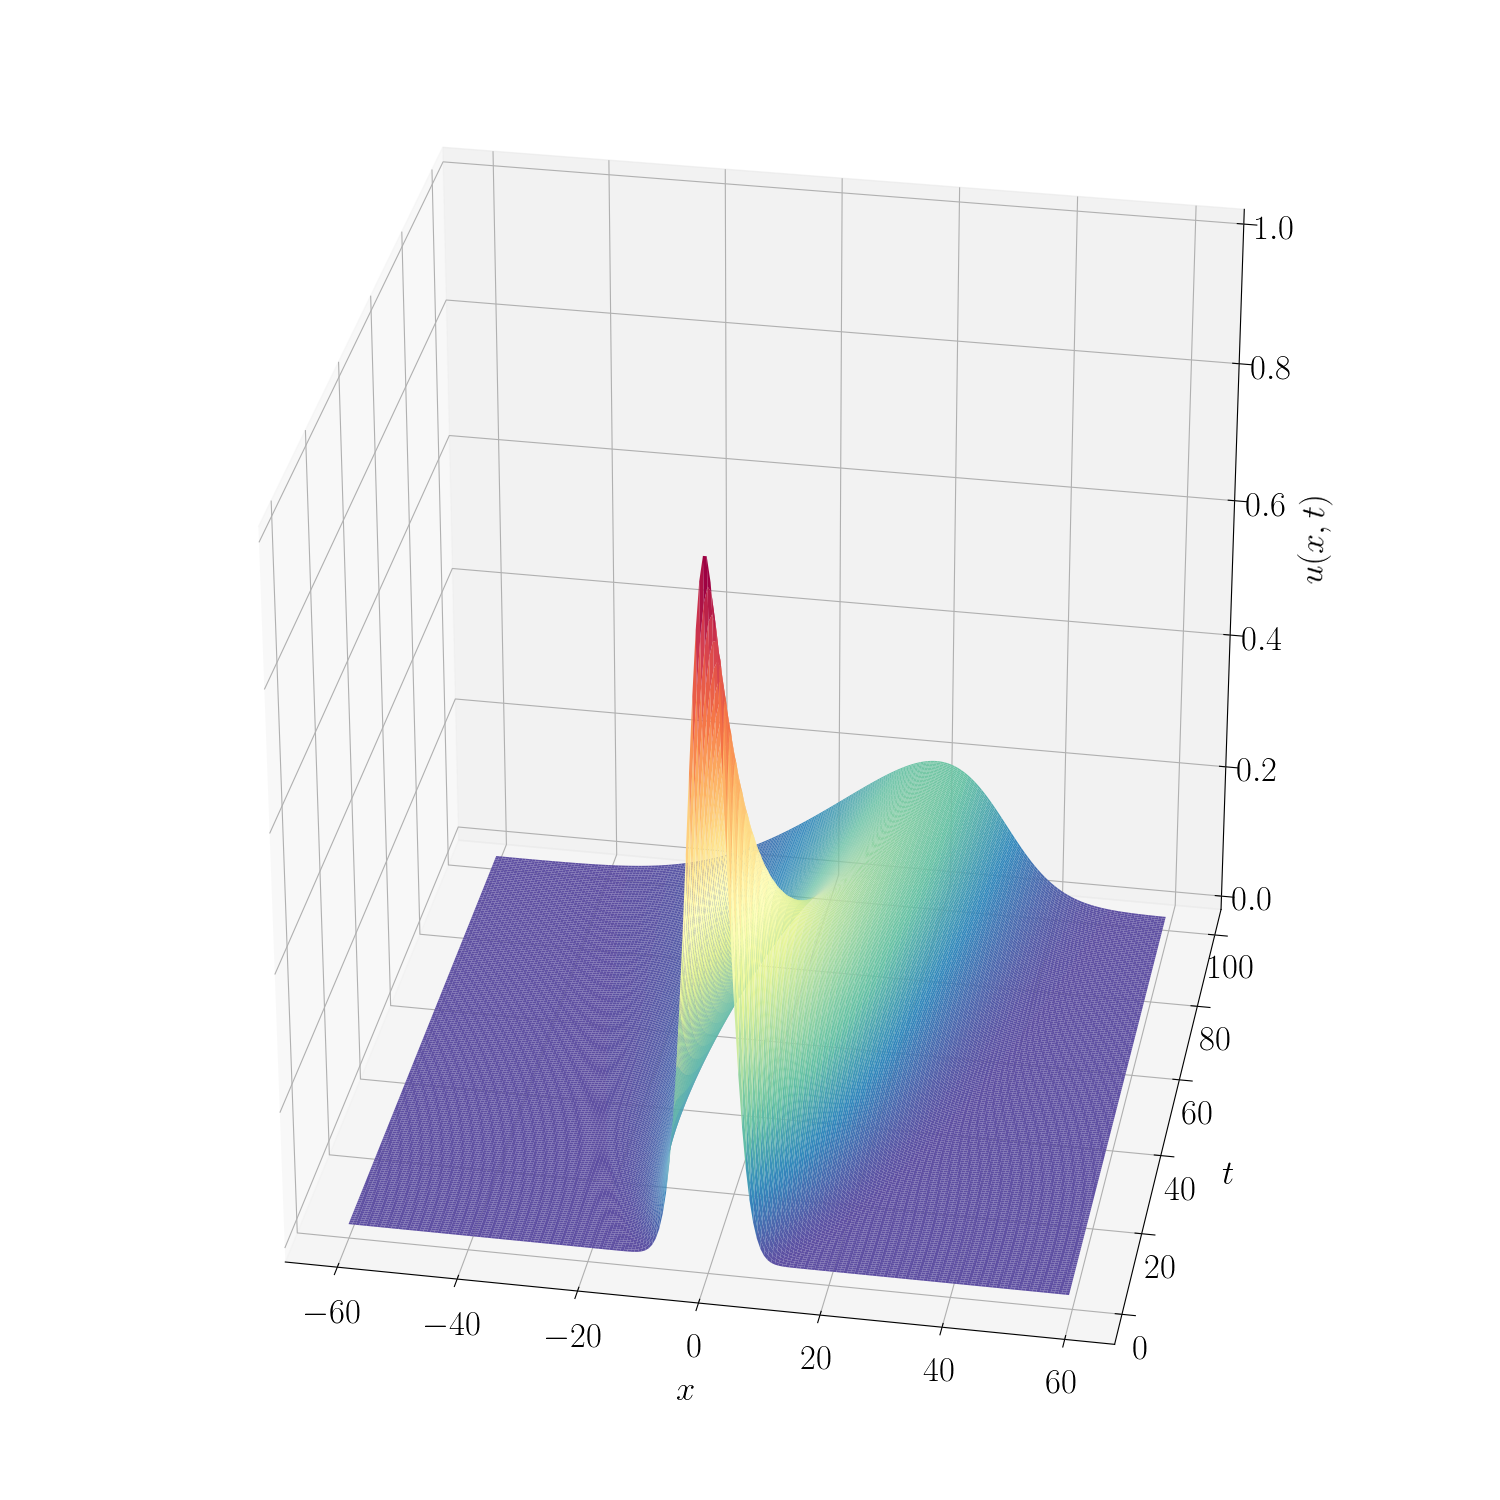
\includegraphics[width=12cm]{burgers_equation/deterministic/numerical_experiments/viscid/figures/collocation/Numerical_Solution_alpha=1.png}
		\label{Collocation_alpha=1}
		\caption{Numerical solution for (\ref{IVP_Burgers}) using (\ref{Collocation_Euler}) at the time $T = 100$ with $\alpha = 1.0$, and $\Delta t = 1.0 \times 10^{-5}$. (b) Point-wise error of approximation}
		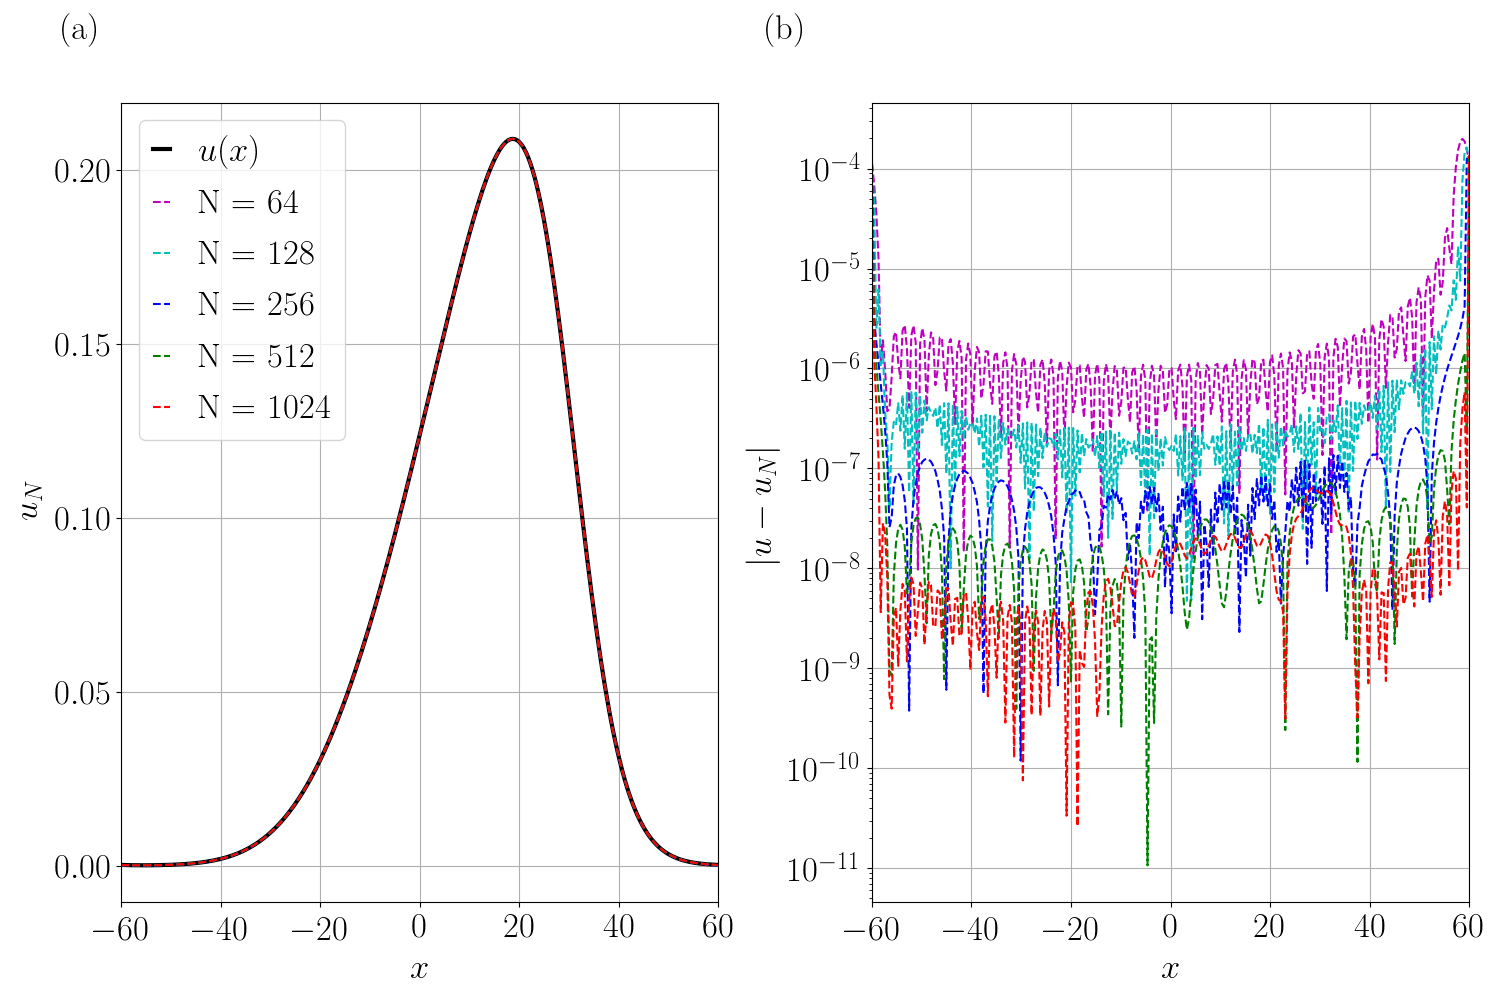
\includegraphics[width=12.5cm]{burgers_equation/deterministic/numerical_experiments/viscid/figures/collocation/Numerical_Solution_alpha=1_T=100.png}
		\label{Collocation_alpha=1_T}
	\end{figure}
	\begin{table}[H]
		\begin{tabular}{lcccc}
			\toprule
			\multicolumn{1}{c}{\textbf{Expansion}} & \multicolumn{4}{c}{\textbf{Error}} \\
			$\hspace{9mm}N$ & $\Delta t=1\times 10^{-2}$ & $\Delta t=1\times 10^{-3}$ & $\Delta t=1\times 10^{-4}$ & $\Delta t=1\times 10^{-5}$ \\
			\midrule
			\hspace{7mm} 16 & 0.721112    & 0.721112    & 0.721112    & 0.721112    \\
			\midrule
			\hspace{7mm} 32 & 4.71797 $\times 10^{-2}$   & 4.72892 $\times 10^{-2}$   & 4.73004 $\times 10^{-2}$   & 4.73015 $\times 10^{-2}$   \\
			\midrule
			\hspace{7mm} 64 & 1.17954 $\times 10^{-3}$  & 7.35344 $\times 10^{-4}$ & 7.27561 $\times 10^{-4}$ & 7.27283 $\times 10^{-4}$  \\
			\midrule
			\hspace{7mm} 128 & 9.43454 $\times 10^{-4}$ & 1.75152 $\times 10^{-4}$ & 1.74583 $\times 10^{-4}$ & 1.74574 $\times 10^{-4}$ \\
			\midrule
			\hspace{7mm} 256 & 9.43454 $\times 10^{-4}$ & 1.15509 $\times 10^{-4}$ & 1.14669 $\times 10^{-4}$ & 1.14659 $\times 10^{-4}$ \\
			\midrule
			\hspace{7mm} 512 & 9.43454 $\times 10^{-4}$ & 9.41793 $\times 10^{-5}$ & 7.78847 $\times 10^{-5}$ & 7.78707 $\times 10^{-5}$ \\
			\midrule
			\hspace{7mm} 1024 & $\ast$         & 9.41793 $\times 10^{-5}$ & 5.32213 $\times 10^{-5}$ & 5.32019 $\times 10^{-5}$ \\
			\midrule
			\hspace{7mm} 2048 & $\ast$           & $\ast$           & 3.56779 $\times 10^{-5}$ & 3.56498 $\times 10^{-5}$ \\
			\\
			\bottomrule
		\end{tabular}
		\caption{Error using $L^2$-norm with $\alpha=1.0$}
		\label{Collocation_tabla_L2_alpha=1}
		\vspace{1cm}
		\begin{tabular}{lcccc}
			\toprule
			\multicolumn{1}{c}{\textbf{Expansion}} & \multicolumn{4}{c}{\textbf{Error}} \\
			$\hspace{9mm}N$ & $\Delta t=1\times 10^{-2}$ & $\Delta t=1\times 10^{-3}$ & $\Delta t=1\times 10^{-4}$ & $\Delta t=1\times 10^{-5}$ \\
			\midrule
			\hspace{7mm} 16 & 0.317617    & 0.317617    & 0.317617    & 0.317617    \\
			\midrule
			\hspace{7mm} 32 & 1.95279 $\times 10 ^{-2}$  & 1.96812 $\times 10 ^{-2}$   & 1.96965 $\times 10 ^{-2}$   & 1.96981 $\times 10 ^{-2}$   \\
			\midrule
			\hspace{7mm} 64 & 6.21793 $\times 10 ^{-4}$ & 2.9813 $\times 10 ^{-4}$  & 2.80086 $\times 10 ^{-4}$ & 2.78934 $\times 10 ^{-4}$ \\
			\midrule
			\hspace{7mm} 128 & 4.74952 $\times 10 ^{-4}$ & 1.64746 $\times 10 ^{-4}$ & 1.6473 $\times 10 ^{-4}$  & 1.64728 $\times 10 ^{-4}$ \\
			\midrule
			\hspace{7mm} 256 & 4.74936 $\times 10 ^{-4}$ & 1.52482 $\times 10 ^{-4}$ & 1.52467 $\times 10 ^{-4}$ & 1.52465 $\times 10 ^{-4}$ \\
			\midrule
			\hspace{7mm} 512 & 4.74936 $\times 10 ^{-4}$ & 1.47249 $\times 10 ^{-4}$ & 1.47234 $\times 10 ^{-4}$ & 1.47232 $\times 10 ^{-4}$ \\
			\midrule
			\hspace{7mm} 1024 & $\ast$           & 1.45032 $\times 10 ^{-4}$ & 1.45017 $\times 10 ^{-4}$ & 1.45016 $\times 10 ^{-4}$ \\
			\midrule
			\hspace{7mm} 2048 & $\ast$           & $\ast$           & 1.43941 $\times 10 ^{-4}$ & 1.4394 $\times 10 ^{-4}$ \\
			\\
			\bottomrule
		\end{tabular}
		\caption{Error using Max norm with $\alpha=1.0$}
		\label{Collocation_tabla_max_alpha=1}
	\end{table}
	
	
	\begin{figure}[H]
		\centering
		\caption{Numerical solution for (\ref{IVP_Burgers}) using (\ref{Collocation_Euler}) with $\alpha = 0.005$, $N=2048$, and $\Delta t = 1.0 \times 10^{-5}$.}
		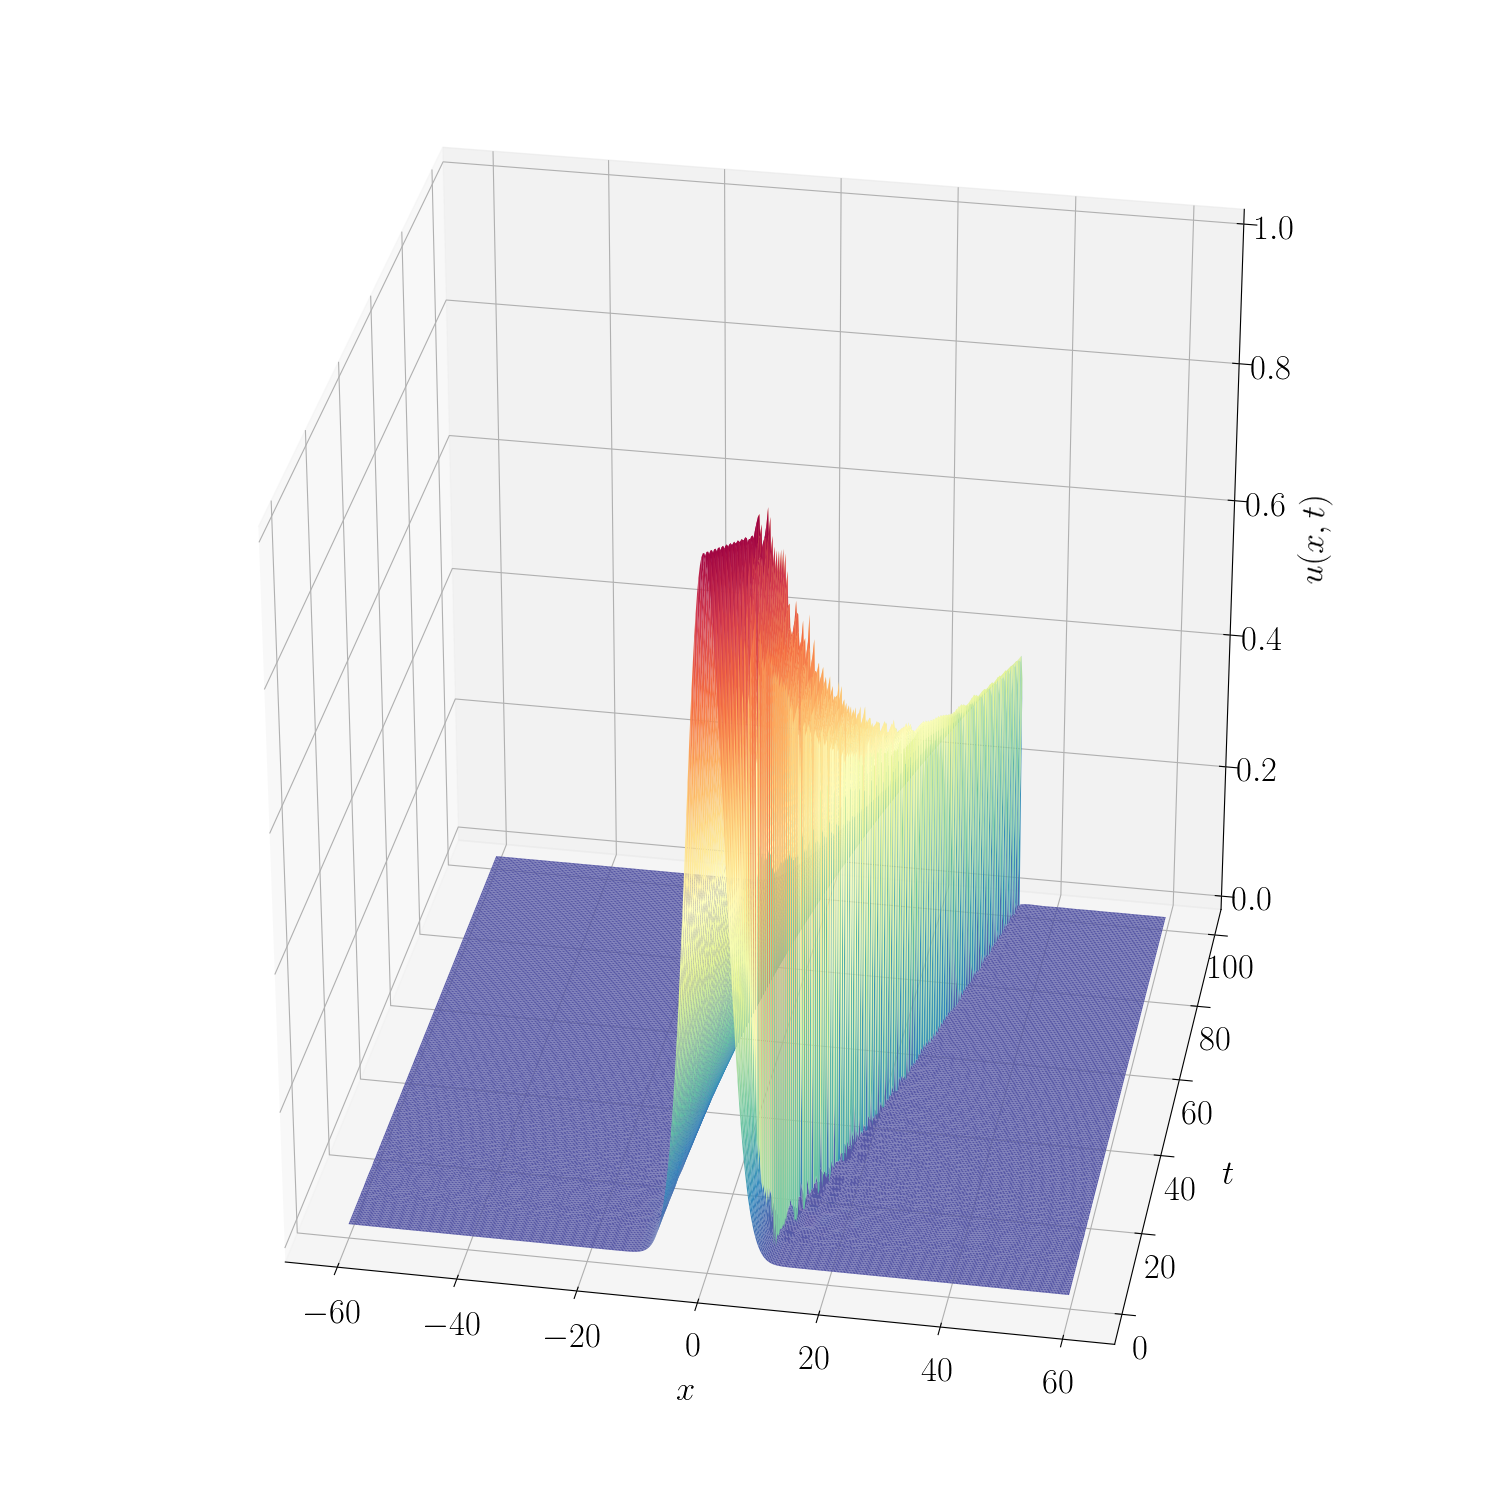
\includegraphics[width=12cm]{burgers_equation/deterministic/numerical_experiments/viscid/figures/collocation/Numerical_Solution_alpha=0005.png}
		\label{Collocation_alpha=005}
		\caption{Numerical solution for (\ref{IVP_Burgers}) using (\ref{Collocation_Euler}) at the time $T = 100$ with $\alpha = 0.005$, and $\Delta t = 1.0 \times 10^{-5}$. (b) Point-wise error of approximation.}
		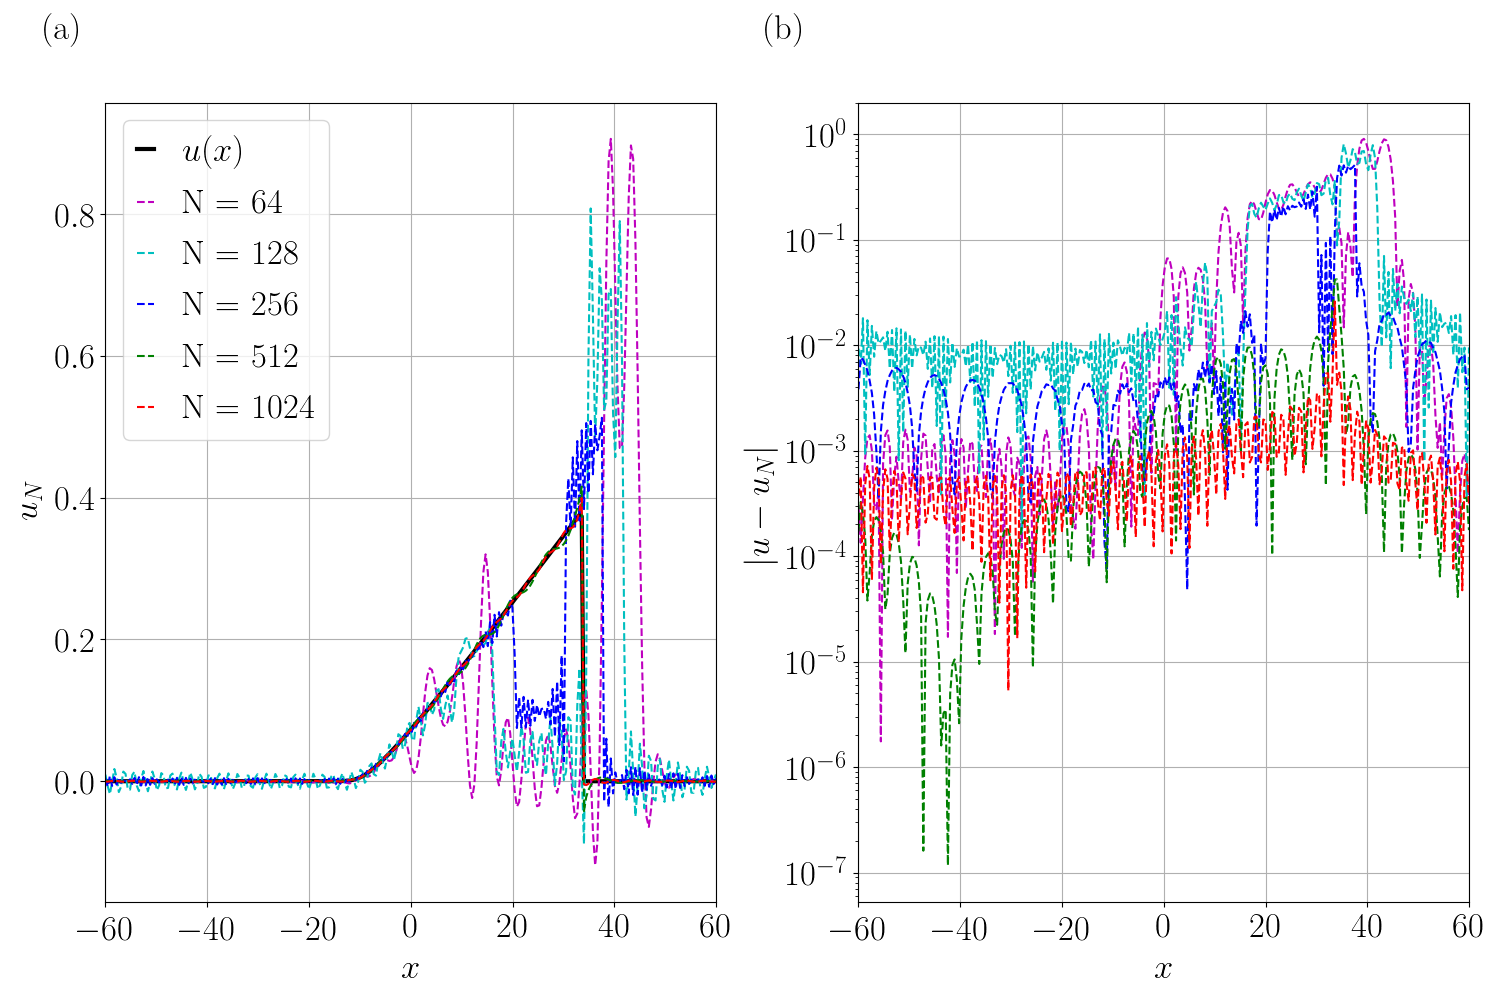
\includegraphics[width=12.5cm]{burgers_equation/deterministic/numerical_experiments/viscid/figures/collocation/Numerical_Solution_alpha=0005_T=100.png}
		\label{Collocation_alpha=005_T}
	\end{figure}
	%L2
	
	\begin{table}[H]
	\begin{tabular}{lcccc}
		\toprule
		\multicolumn{1}{c}{\textbf{Expansion}} & \multicolumn{4}{c}{\textbf{Error}} \\
		$\hspace{9mm}N$ & $\Delta t=1\times 10^{-2}$ & $\Delta t=1\times 10^{-3}$ & $\Delta t=1\times 10^{-4}$ & $\Delta t=1\times 10^{-5}$ \\
		\midrule
		\hspace{7mm} 16 & 1.36189   & 1.35883    & 1.35852   & 1.35849   \\
		\midrule
		\hspace{7mm} 32 & 2.67506   & 2.65305    & 2.65078   & 2.65055   \\
		\midrule
		\hspace{7mm} 64 & 2.50365   & 2.45855    & 2.45432   & 2.45387   \\
		\midrule
		\hspace{7mm} 128 & 2.15795   & 2.0632     & 2.05589   & 2.05497   \\
		\midrule
		\hspace{7mm} 256 & 1.362     & 1.18393    & 1.16697   & 1.16532   \\
		\midrule
		\hspace{7mm} 512 & 0.350775  & 0.304595   & 0.300865  & 0.300499  \\
		\midrule
		\hspace{7mm} 1024 & 0.168462  & 0.140332   & 0.13803   & 0.137804  \\
		\midrule
		\hspace{7mm} 2048 & 6.56161 $\times 10^{-2}$ & 4.63808 $\times 10^{-2}$  & 4.49226 $\times 10^{-2}$ & 4.47813 $\times 10^{-2}$ \\
		\\
		\bottomrule
	\end{tabular}
	\caption{Error using $L^2$-norm with $\alpha=0.005$}
	\label{Collocation_tabla_L2_alpha=005}
	\vspace{1cm}
	\begin{tabular}{lcccc}
		\toprule
		\multicolumn{1}{c}{\textbf{Expansion}} & \multicolumn{4}{c}{\textbf{Error}} \\
		$\hspace{9mm}N$ & $\Delta t=1\times 10^{-2}$ & $\Delta t=1\times 10^{-3}$ & $\Delta t=1\times 10^{-4}$ & $\Delta t=1\times 10^{-5}$ \\
		\midrule
		\hspace{7mm} 16 & 0.695784 & 0.695659  & 0.695646  & 0.695645 \\
		\midrule
		\hspace{7mm} 32 & 1.20278  & 1.19418   & 1.19329   & 1.1932   \\
		\midrule
		\hspace{7mm} 64 & 1.22454  & 1.18903   & 1.18507   & 1.18467  \\
		\midrule
		\hspace{7mm} 128 & 1.11999  & 1.0238    & 1.01754   & 1.01701  \\
		\midrule
		\hspace{7mm} 256 & 0.927954 & 0.877058  & 0.872508  & 0.87201  \\
		\midrule
		\hspace{7mm} 512 & 0.664133 & 0.415288  & 0.39714   & 0.395563 \\
		\midrule
		\hspace{7mm} 1024 & 0.247742 & 0.259451  & 0.260605  & 0.26072  \\
		\midrule
		\hspace{7mm} 2048 & 0.126824 & 0.103297  & 0.107102  & 0.10748  \\
		\\
		\bottomrule
	\end{tabular}
	\caption{Error using Max norm with $\alpha=0.005$}
	\label{Collocation_tabla_max_alpha=005}
	\end{table}
	\subsection{Numerical Solutions for Burgers' Equation without Viscosity}
	
	To finish the section, we will study the problem (\ref{IVP_Burgers}) without viscosity, that is, when $\alpha = 0$. So the problem is the following
	\begin{align}
	\label{IVP_Inviscid}
		\left \lbrace \begin{array}{ll}
			\frac{\partial u}{\partial t} + \frac{1}{2} (u^2)_x = 0, \hspace{2mm} 0 < t \leq T, \hspace{2mm} x \in \mathcal{D} \\
			\\
			u(x, 0) = u_0(x), \hspace{2mm} x \in \mathcal{D}
		\end{array}  \right .
	\end{align}

	This problem, which seems much simpler, turns out to be very interesting, because it presents relevant characteristics regarding the physical interpretation of the problem in general, that is, the case with non-zero viscosity. \\
	
	The previous equation interprets the conservation of energy and is considered as a non-linear conservation law. We can understand this if we consider the function $ u $ as the speed of a fluid that conserves its energy with a flow density given by $f(u) = \frac{u^2} {2}$. \\
	
	The above can be shown considering that $u \in H^1_p [\mathcal{D}]$, and multiplying by $u$ and integrating both sides of the equation on the domain $\mathcal{D}$ to prove that $\| u \|$ does not change over time, that is,
	\begin{align*}
		\frac{1}{2} \frac{d}{dt} \displaystyle \int_{0}^{2 \pi} u^2(x, t) dx = - \int_{0}^{2 \pi} u^2(x, t) \frac{\partial u(x, t)}{\partial x} dx = - \frac{1}{3} u^3(x, t) \Big|^{2 \pi}_{0}.
	\end{align*}
	and because $u$ is periodic, we have to
	\begin{align*}
		\frac{1}{2} \frac{d}{dt} \| u(x, t) \|^2 = 0.
	\end{align*}
	This means that the energy is conserved with the same initial energy since we must bear in mind that this represents the kinetic energy of a fluid that travels with a velocity given by $u_0$. \\
		
	In any problem, these characteristics are of utmost importance, this is because we must consider the behavior of the solutions when they must be approached with some numerical method. In the literature, when a solution remains bounded in time, the problem is said to be well defined. In the analysis context, this assures us the existence of a continuously differentiable solution $u$, and that besides being unique, it is possible to approximate it. \\
	
	However, approximating the solutions to this problem using spectral methods can be more complicated if its characteristics are not well understood. Next, we will see that under a certain condition it is possible to find a single analytical solution and that otherwise, it may lose its uniqueness when developing discontinuities. \\
			
	First, let's define the curves $x = x(t)$ that start at a point $x_0 \in \mathbb{R}$, and satisfy the following problem
	\begin{align*}
		\left \lbrace \begin{array}{ll}
			x' (t) = u(x(t), t), \hspace{2mm} t > 0, \\
			\\
			x(0) = x_0.
		\end{array} \right .  
	\end{align*}
	
	The solutions for each $x_0$ are known as characteristic curves, which pass through the solution $u = u (x (t), t)$. It is well known in the theory of differential equations that when $u(x, t)$ is locally Lipschitz in the variable $x$, and continues in the variable $t$, the above equation admits a single solution $x(t)$ for each $x_0 \in \mathbb{R}$. So, assuming the above we have that for a solution $ x (t) $ corresponding to a fixed $x_0 \in \mathbb{R}$, it satisfies the following
	\begin{align*}
		\frac{d}{dt} [u(x(t), t)] &= x' (t) u_x (x(t), t) + u_t (x(t), t) \\
		&= u(x(t), t) u_x (x(t), t) - u(x(t), t) u_x (x(t), t) = 0
	\end{align*}
	which tells us that the function $u(x (t), t)$ is independent of the variable $t$, remaining constant along the characteristic curve. Therefore, we have to
	\begin{align*}
		u(x(t), t) = u (x(0), 0) = u_0 (x_0)
	\end{align*}
	
	Furthermore, we have that the solution $ x (t) $ will be given by the following curve
	\begin{align*}
		x(t) = x_0 + u_0 (x_0) t, \hspace{2mm} t > 0.
	\end{align*}
	which allows us to write the solution $ u(x, t)$ as follows
	\begin{align}
	\label{Exact_Inviscid}	
		u(x, t) = u_0(x_0), \hspace{2mm} x_0 = x - u_0(x_0) t
	\end{align}
	
	Note that the Lipschitz condition is necessary for the uniqueness of the above solution, since, conversely, if we set two different starting points $x_0, x_1$ such that $x_0 <x_1$, then its curves characteristics intersect for some $t$, that is,
	\begin{align*}
		x_0 + u_0(x_0) t = x_1 + u_0 (x_1) t,
	\end{align*}
	and using the mean value theorem we have that for some $c \in (x_0, x_1)$ the time $t$ is given by
	\begin{align*}
		t = \frac{x_1 - x_0}{u_0 (x_0) - u_0 (x_1)} = - \frac{1}{u'_0(c)},
	\end{align*}
	
	The above tells us that when these two curves intersect, the solution $u (x, t)$ cannot be continuous in the time $ t $ given by the previous equation. This is because $u_0 (x_0) \neq u_0 (x_1)$, and since the solution is constant over time we would have that $u (x, t) = u_0 (x_0) = u_0 (x_1)$, which is impossible. \\
		
	Therefore, the time $t$ for which two curves intersect represents a discontinuity, and that can be calculated by
	\begin{align}
	\label{shock_time}	
			Tc = \min_{x \in \mathbb{R}} \left[  \frac{-1}{u'_0 (x)} \right]
	\end{align}
	and we can observe that the continuity of the solution $u$ is assured if $T_c < 0$, which depends only on the initial condition $u_0$. \\
	
	This type of information allows us to know the criteria that must be considered when implementing numerical methods, but also the physical interpretation of the problem can be useful. For example, the solution to this problem can be considered to simulate the evolution of the profile of a sea wave that deforms as it approaches the coast until it breaks. But when this occurs, the deformation of the wave stops precisely at the time $T_c$. \\
	
	We must consider that the problem without viscosity supposes that the fluid behaves in an ideal or perfect way, traveling as if they were separate sheets without rubbing. But in real life, fluids always have a certain degree of viscosity, that is, the fluid sheets can rub and cause energy dissipation, and for these cases, we could consider the problem with sufficiently small values ​​of $\alpha$. So a question that naturally arises is what the behavior of the solutions looks like when $\alpha$ approaches zero. \\
	
	In chapter \ref{Introduction} we obtained the solution of the problem (\ref{IVP_Burgers}), which is given by (\ref{Exact_Solution}), and from this equation we can see that the solutions are infinitely differentiable for any value of $\alpha> 0$. Instinctively, we can notice that the solution approaches the solution of the equation without viscosity when $\alpha$ approaches zero. In fact, the solution obtained as a limit when $\alpha$ approaches zero is known as the entropy solution, which has been studied in \cite{Tadmor1989}, \cite{Maday1989} and in \cite{Kruzkov1970} has been proved that this solution is unique. \\
	
	In order to illustrate what we have previously discussed, we will consider the problem (\ref{IVP_Inviscid}) with the following initial condition function
	\begin{align}
	\label{IC_Inviscid}	
		u_0 (x) = e^{-0.005x^2}, \hspace{3mm} x \in \mathcal{D}
	\end{align}
	where $\mathcal{D} = [x_L, x_R]$, and considering the interval $I = [0, T_c]$ for a value of $T_c$ given by (\ref{shock_time}). \\
	
	In the following simulations, we will use the Fourier-Galerkin method given in (\ref{Galerkin_Euler}) to obtain approximations with different values of $\alpha$, and we will see how they approximate the exact solution of the problem (\ref{IC_Inviscid} ) which was given in (\ref {Exact_Inviscid}).
	
	\newpage
	\begin{figure}[H]
		\centering
		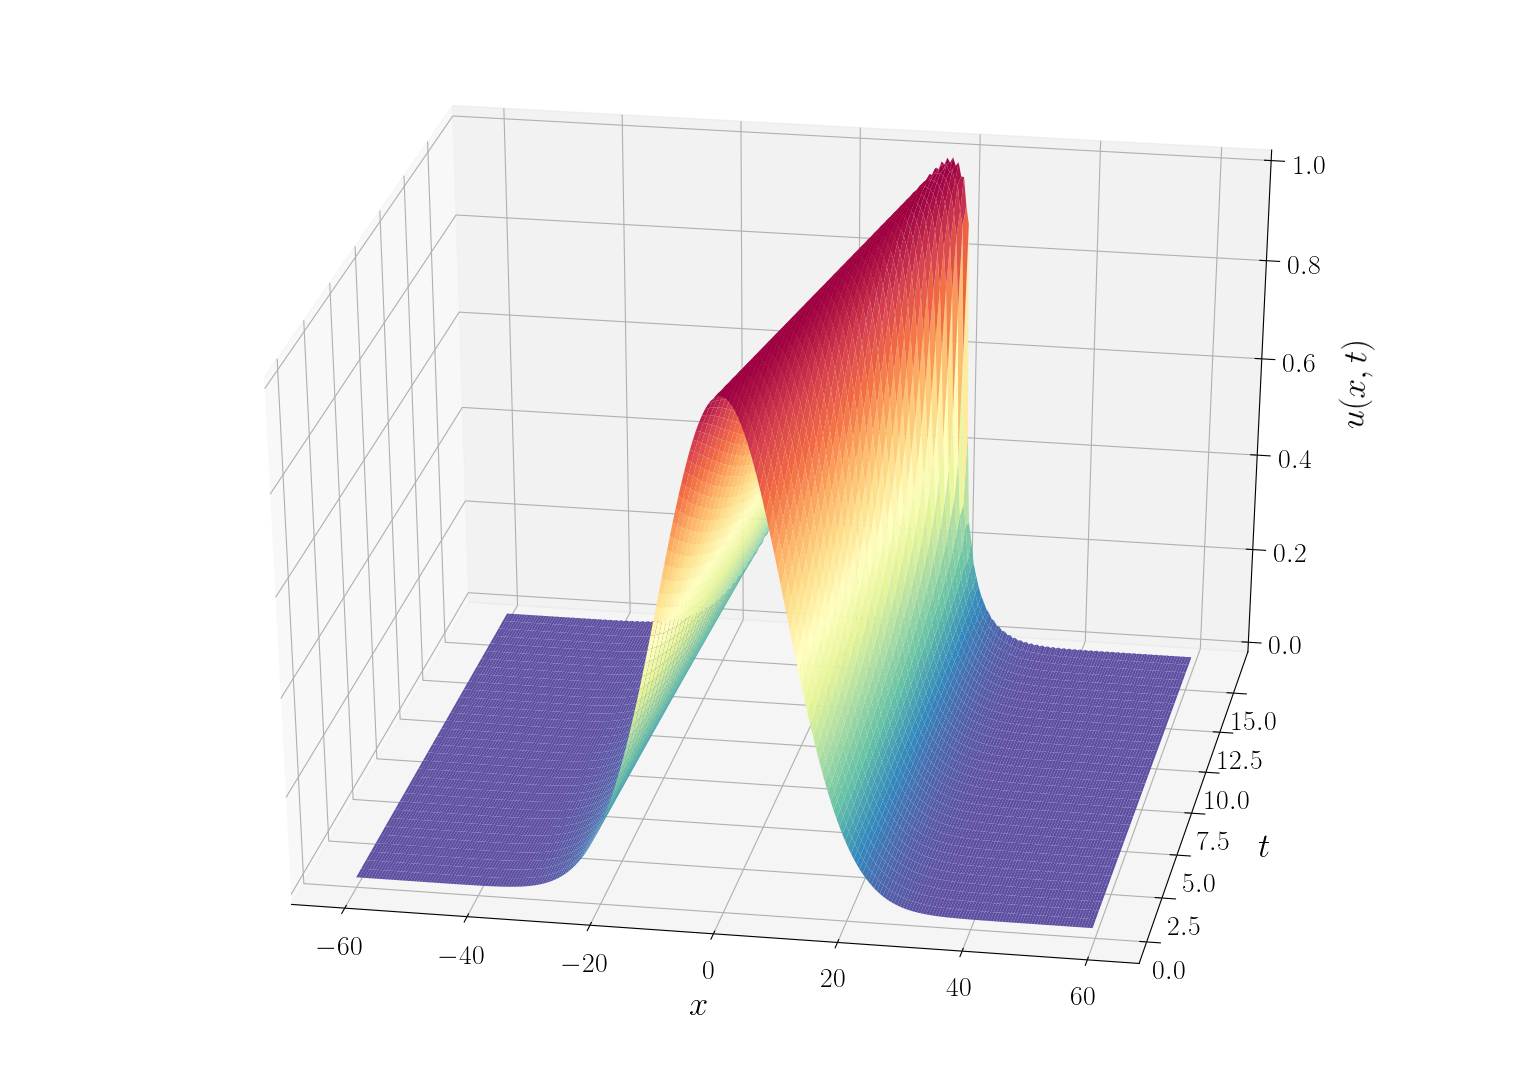
\includegraphics[width=12cm]{burgers_equation/deterministic/numerical_experiments/inviscid/figures/small_alpha.png}
		\caption{Numerical solution for (\ref{IVP_Burgers}) using (\ref{Galerkin_Euler}) with $\alpha = 1.0 \times 10^{-5}$, $N=256$, and $\Delta t = 1.0 \times 10^{-3}$.}
		\vspace{2mm}
		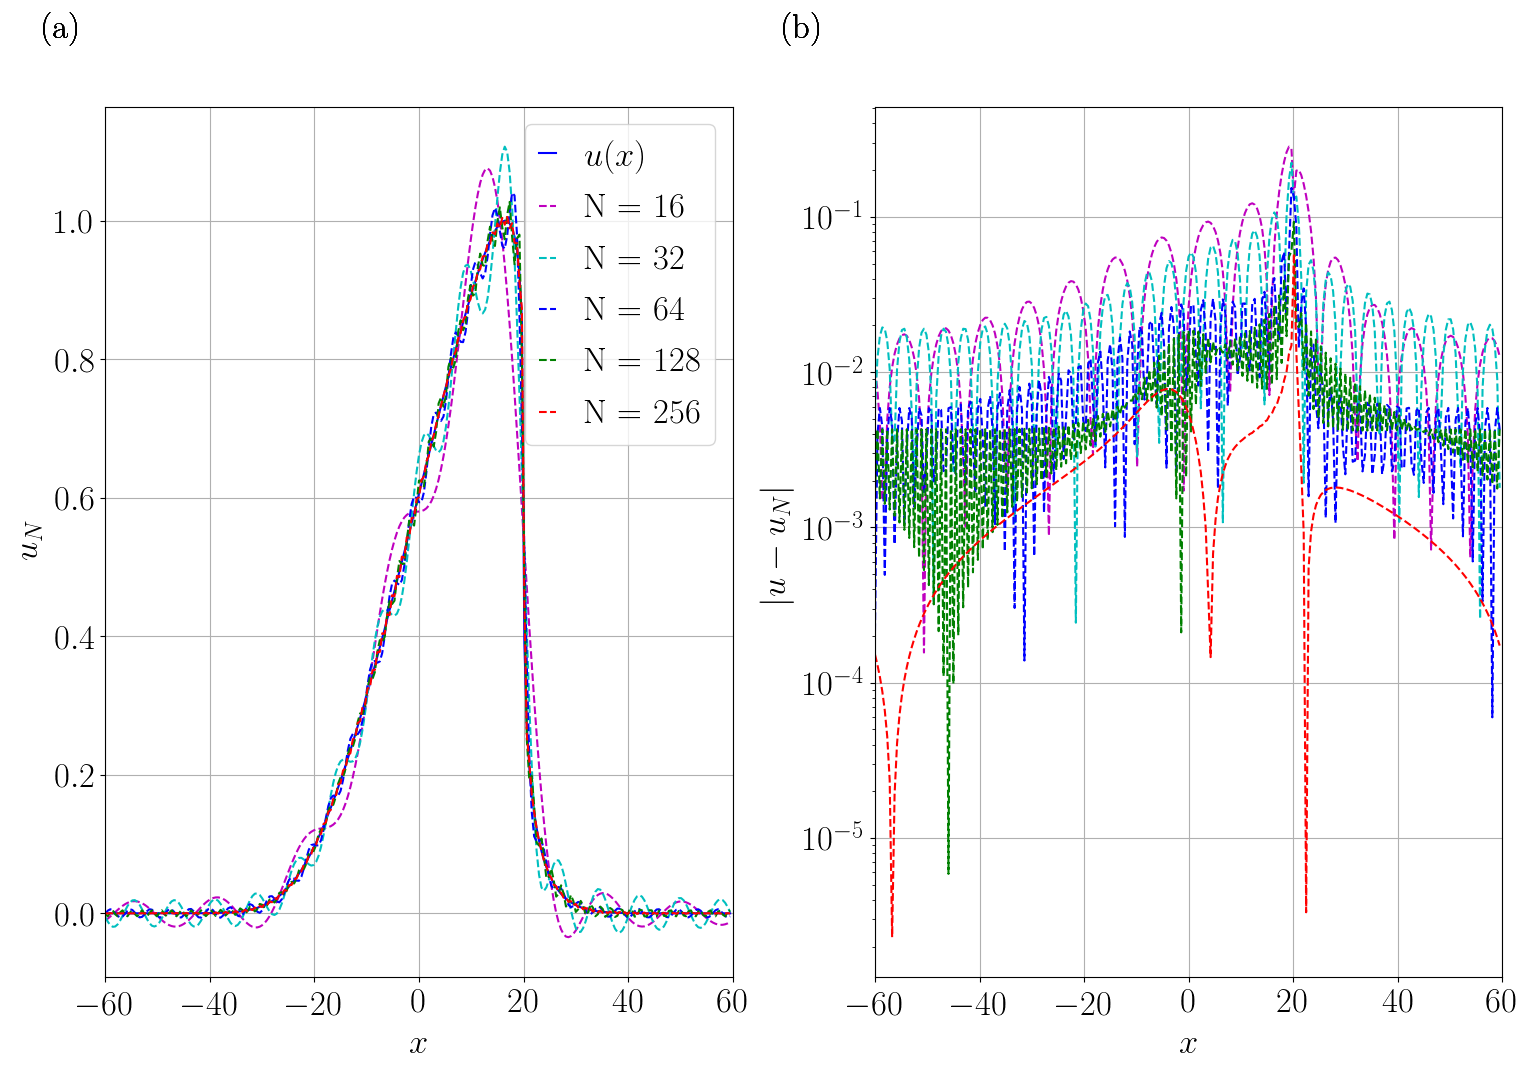
\includegraphics[width=12.5cm]{burgers_equation/deterministic/numerical_experiments/inviscid/figures/small_alpha_T.png}
		\caption{Numerical solution for (\ref{IVP_Burgers}) using (\ref{Galerkin_Euler}) at the time $T_c$ with $\alpha = 1.0 \times 10^{-5}$, and $\Delta t = 1.0 \times 10^{-3}$. (b) Point-wise error of approximation.}
	\end{figure}
	\newpage
	\begin{figure}[H]
		\centering	
		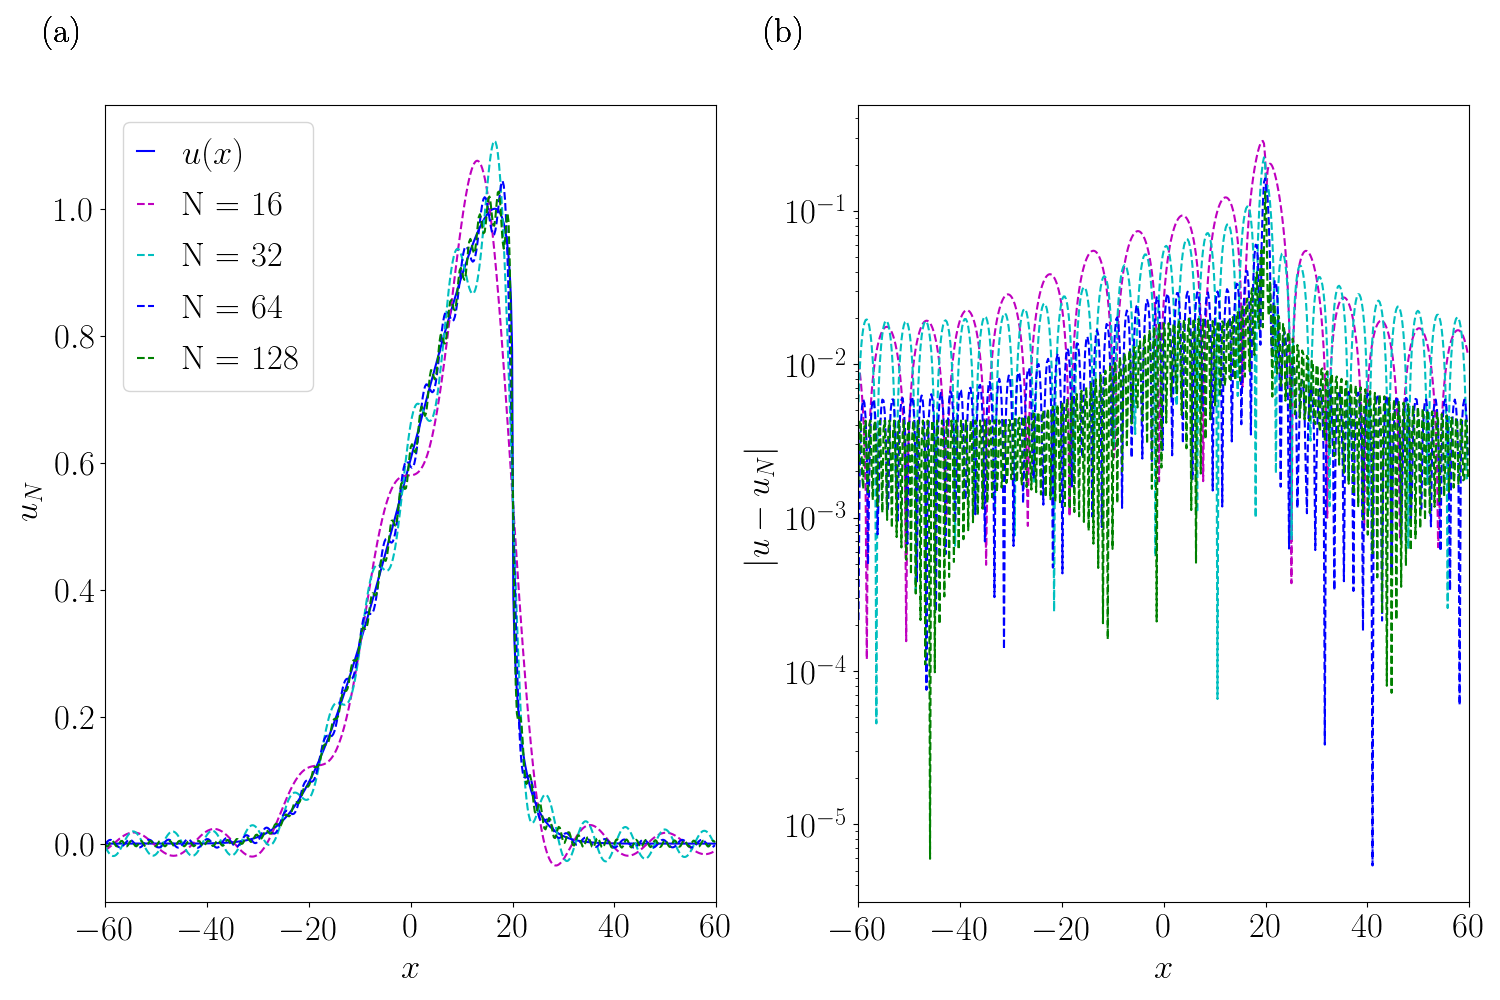
\includegraphics[width=13cm]{burgers_equation/deterministic/numerical_experiments/inviscid/figures/Numerical_Solution_Inviscid_T.png}
		\caption{(a) Exact solution for (\ref{IVP_Burgers}), and its approximations using (\ref{Galerkin_Euler}) at the time $Tc$ with initial condition $u_0(x) = e^{-0.005x^2}$, $x \in [-60, 60]$. (b) Pointwise error of approximation.}
		\label{convection_aprox_T}
		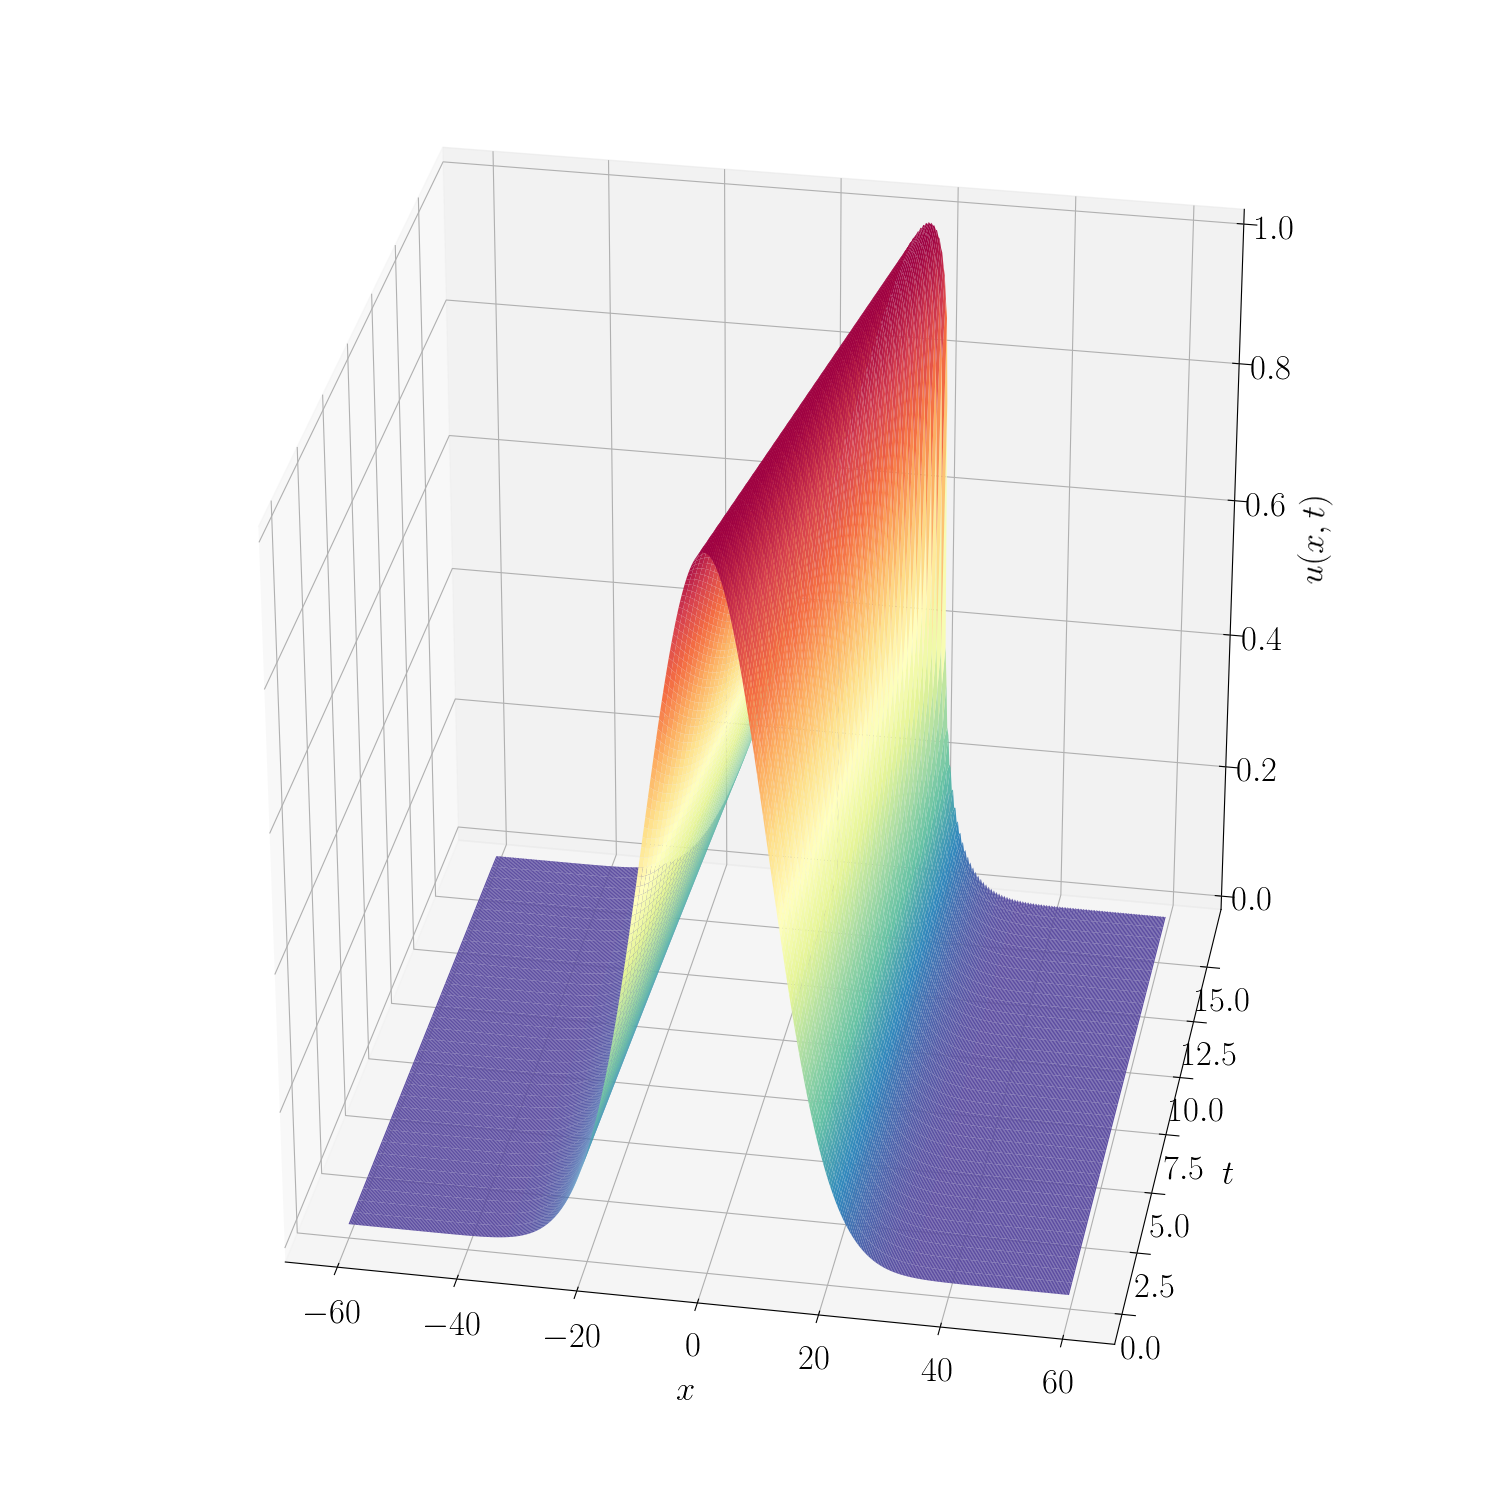
\includegraphics[width=11cm]{burgers_equation/deterministic/numerical_experiments/inviscid/figures/Numerical_Solution_Inviscid.png}
		\caption{Numerical approximation for  \ref{IVP_Burgers} using (\ref{Galerkin_Euler}) with $N=512$, $u_0(x) = e^{-0.005x^2}$, $x \in [-60, 60]$, and $t \in [0, Tc]$.}
	\end{figure}
	\newpage
	\begin{table}[H]
		\centering
		\begin{tabular}{lccc}
			\toprule
			\multicolumn{1}{c}{\hspace{6mm}\textbf{Expansion}} & \multicolumn{3}{c}{\textbf{Distance}} \\
			\hspace{12mm} $N$ & $\Delta t=1\times 10^{-2}$ & $\Delta t=1\times 10^{-3}$ & $\Delta t=1\times 10^{-4}$ \\
			\midrule
			\hspace{12mm} 16 & 0.285531 & 0.285732 & 0.285752 \\
			\midrule
			\hspace{12mm} 32 & 0.222737 & 0.223260 & 0.223312 \\
			\midrule
			\hspace{12mm} 64 & 0.160385 & 0.162782 & 0.163025 \\
			\midrule
			\hspace{12mm} 128 & 0.129297 & 0.133322 & 0.133733 \\
			\midrule
			\hspace{12mm} 256 & 0.083291 & 0.091449 & 0.092320 \\
			\bottomrule
		\end{tabular}
		\caption{Distance between exact solution for (\ref{IVP_Inviscid}) and the approximation for (\ref{IVP_Burgers}) with $\alpha = 1.0 \times 10^{-5}$.}
	\end{table}
	\begin{figure}[H]
		\centering
		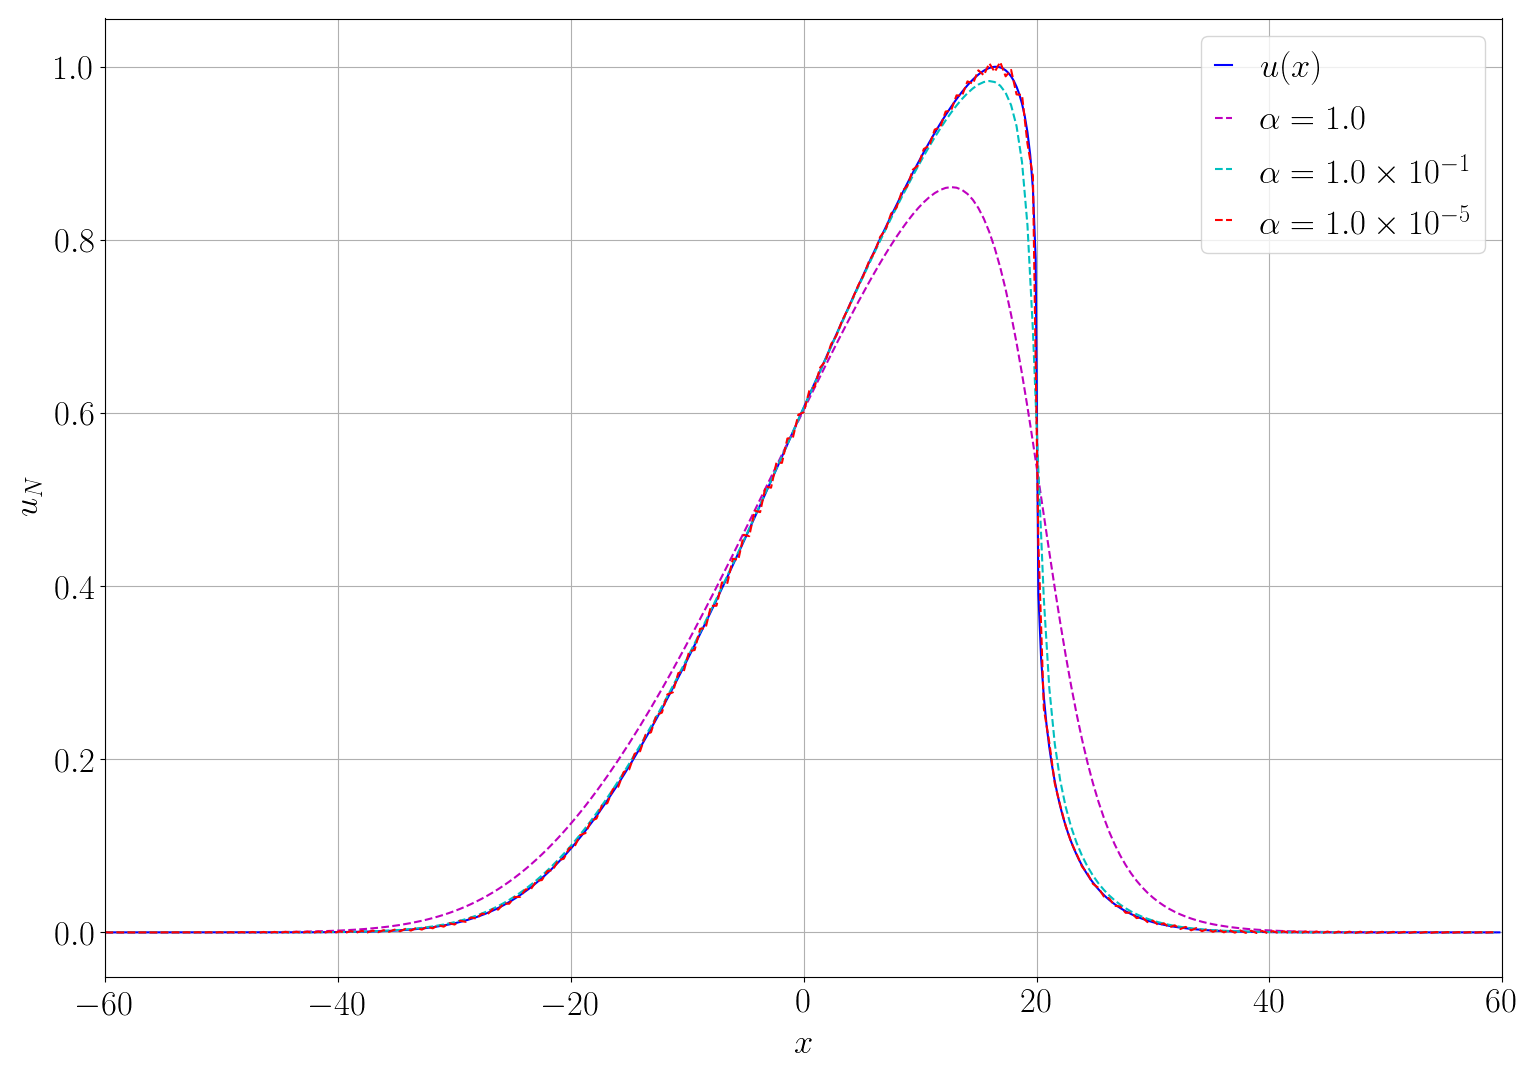
\includegraphics[width=12cm]{burgers_equation/deterministic/numerical_experiments/inviscid/figures/varios_alphas.png}
		\caption{Exact solution for (\ref{IVP_Inviscid}) and different approximations using (\ref{Galerkin_Euler}) with $N=256$, and $\Delta t = 1.0 \times 10^{-3}$.}
	\end{figure}